\documentclass[12pt,openany]{book}
\usepackage{kotex}
\usepackage{amsmath,amsthm,amsfonts,amscd} % Packages for mathematics
\usepackage{commath} %absolute value
% Colors
\usepackage[dvipsnames]{xcolor}
\definecolor{titleblue}{RGB}{0,53,128}
\definecolor{chaptergray}{RGB}{140,140,140}
\definecolor{sectiongray}{RGB}{180,180,180}

\definecolor{thmcolor}{RGB}{231, 76, 60}
\definecolor{defcolor}{RGB}{52, 152, 219}
\definecolor{lemcolor}{RGB}{155, 89, 182}
\definecolor{corcolor}{RGB}{46, 204, 113}
\definecolor{procolor}{RGB}{241, 196, 15}

% Fonts
\usepackage[T1]{fontenc}
\usepackage[utf8]{inputenc}
\usepackage{newpxtext,newpxmath}
\usepackage{sectsty}
\allsectionsfont{\sffamily\color{titleblue}\mdseries}

% Page layout
\usepackage{geometry}
\geometry{a4paper,left=1in,right=.7in,top=1in,bottom=1in,heightrounded}
\usepackage{fancyhdr}
\fancyhf{}
\fancyhead[LE,RO]{\thepage}
\fancyhead[LO]{\nouppercase{\rightmark}}
\fancyhead[RE]{\nouppercase{\leftmark}}
\renewcommand{\headrulewidth}{0.5pt}
\renewcommand{\footrulewidth}{0pt}

% Chapter formatting
\usepackage{titlesec}
\titleformat{\chapter}[display]
{\normalfont\sffamily\Huge\bfseries\color{titleblue}}{\chaptertitlename\ \thechapter}{20pt}{\Huge}
\titleformat{\section}
{\normalfont\sffamily\Large\bfseries\color{titleblue!100!gray}}{\thesection}{1em}{}
\titleformat{\subsection}
{\normalfont\sffamily\large\bfseries\color{titleblue!75!gray}}{\thesubsection}{1em}{}

% Table of contents formatting
\usepackage{tocloft}
\renewcommand{\cftchapfont}{\sffamily\color{titleblue}\bfseries}
\renewcommand{\cftsecfont}{\sffamily\color{chaptergray}}
\renewcommand{\cftsubsecfont}{\sffamily\color{sectiongray}}
\renewcommand{\cftchapleader}{\cftdotfill{\cftdotsep}}

\usepackage{cancel}
\newcommand\crossout[3][black]{\renewcommand\CancelColor{\color{#1}}\cancelto{#2}{#3}}
\newcommand\ncrossout[2][black]{\renewcommand\CancelColor{\color{#1}}\cancel{#2}}
% Hyperlinks
\usepackage{hyperref}
\hypersetup{
	colorlinks=true,
	linkcolor=titleblue,
	filecolor=black,      
	urlcolor=titleblue,
}

%Ceiling and Floor Function
\usepackage{mathtools}
\DeclarePairedDelimiter{\ceil}{\lceil}{\rceil}
\DeclarePairedDelimiter{\floor}{\lfloor}{\rfloor}

%Algorithm
\usepackage[ruled,linesnumbered]{algorithm2e}
\usepackage{setspace}
\usepackage{algpseudocode}
\SetKwComment{Comment}{/* }{ */}
\SetKw{Break}{break}
\SetKw{Downto}{downto}
\SetKwProg{Fn}{Function}{:}{end}
\SetKwFunction{KeyGen}{KeyGen}



%---------------------------My Preamble
\usepackage{marvosym} %Lightning
\usepackage{booktabs}
\usepackage{multicol}
\usepackage{tabularx}
\setlength{\columnsep}{2cm}
\setlength{\columnseprule}{1.25pt}
\usepackage{enumerate}
\usepackage{soul}
\newcommand{\mathcolorbox}[2]{\colorbox{#1}{$\displaystyle #2$}}
\usepackage{graphicx}
\usepackage{tikz}
\usepackage{tikz-cd}
\usetikzlibrary{calc}
\usetikzlibrary{arrows, arrows.meta, positioning, shapes.multipart}
\usetikzlibrary{shapes.geometric, decorations.text}
\usepackage{pgfplots}
\usetikzlibrary{patterns}
\pgfplotsset{compat=newest}
\usepackage{colortbl} % for coloring cells
\usepackage{multirow} % for multirow feature
%Tcolorbox
\usepackage[most]{tcolorbox}
\tcbset{colback=white, arc=5pt}
%\tcbset{enhanced, colback=white,colframe=black,fonttitle=\bfseries,arc=4mm,boxrule=1pt,shadow={2mm}{-1mm}{0mm}{black!50}}
%White box with black text and shadow
%\begin{tcolorbox}[colback=white,colframe=black,fonttitle=\bfseries,title=Black Shadow Box,arc=4mm,boxrule=1pt,shadow={2mm}{-1mm}{0mm}{black!50}]
%	This is a white box with black text and a subtle shadow. The shadow adds some depth and dimension to the box without overpowering the design.
%\end{tcolorbox}

%Theorem
%\newtheorem{axiom}{Axiom}[chapter]
\newtheorem{theorem}{Theorem}[chapter]
\newtheorem{proposition}[theorem]{Proposition}
\newtheorem{corollary}{Corollary}[theorem]
\newtheorem{lemma}[theorem]{Lemma}

\theoremstyle{definition}
\newtheorem{definition}{Definition}[chapter]
\newtheorem{remark}{Remark}[chapter]
\newtheorem{exercise}{Exercise}[chapter]
\newtheorem{example}{Example}[chapter]
\newtheorem*{note}{Note}
\newtheorem*{axiom}{Axiom}

%New Command
\newcommand{\N}{\mathbb{N}}
\newcommand{\Z}{\mathbb{Z}}
\newcommand{\Q}{\mathbb{Q}}
\newcommand{\R}{\mathbb{R}}
\newcommand{\C}{\mathbb{C}}
\newcommand{\E}{\mathbb{E}}
\newcommand{\F}{\mathbb{F}}

\newcommand{\dispsty}{\displaystyle}
\newcommand{\sol}{\textcolor{magenta}{\bf Solution}}
\newcommand{\eg}{\textnormal{e.g.}}
\newcommand{\ie}{\textnormal{i.e.}}
\newcommand{\of}[1]{\left(#1\right)}

\newcommand{\Var}{\text{Var}}
\newcommand{\sd}{\text{sd}}
\newcommand{\mean}[1]{\bar{#1}}
\newcommand{\Cov}{\textit{Cov}}
\newcommand{\Corr}{\textit{Corr}}
\newcommand{\SE}{\text{S.E.}}
\newcommand{\df}{\text{d.f.}}

\newcommand{\markov}[1]{\langle #1\rangle}
\newcommand{\tab}{\hspace{12pt}}

% Stirling's approximation for the gamma function
\newcommand{\stirling}[1]{(sqrt(2*pi*#1)*(#1/exp(1))^#1)}

% Begin document
\begin{document}
	
	% Title page
	\begin{titlepage}
		\begin{center}
			{\Huge\textsf{\textbf{Theory of Random Number Generation}}\par}
			\vspace{0.5in}
			{\Large Ji Yong-Hyeon\par}
			\vspace{1in}
			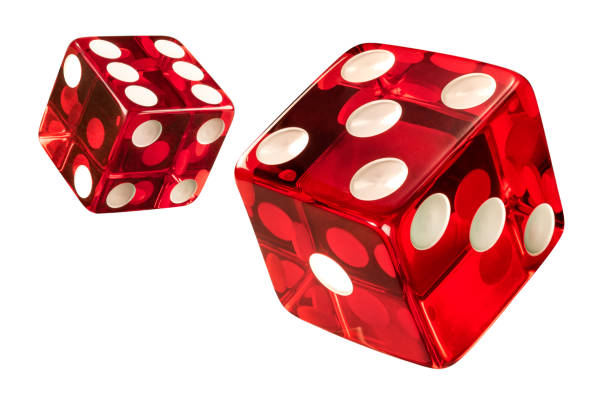
\includegraphics[scale=2]{rng.jpg}\par
			\vspace{1in}\large
			{\bf Department of Information Security, Cryptology, and Mathematics\par}
			{College of Science and Technology\par}
			{Kookmin University\par}
			%\includegraphics[width=1.5in]{school_logo.jpg}\par
			\vspace{.25in}
			{\large \today\par}
		\end{center}
	\end{titlepage}
	
	% Table of contents
	\tableofcontents
	
	% Chapters
	\mainmatter
	
	\chapter{Introduction}
	\begin{tcolorbox}[colback=white,colframe=defcolor,arc=5pt,title={\color{white}\bf Summary}]
		\begin{itemize}
			\item Required Properties for Random Bit Generator
			\begin{itemize}
				\item \textbf{Unpredictability}, \textbf{Unbiasedness}, \textbf{Independence}
			\end{itemize}
			\item Components of Cryptographically Secure Random Bit Generator
			\begin{itemize}
				\item TRNG (Entropy Source) + PRNG (Pseudorandom Number Generator)
			\end{itemize}
			\item Methods for Evaluating the Security of Random Bit Generator
			\begin{itemize}
				\item Estimation of entropy for the output sequence from TRNG
				\item Statistical randomness tests for the output sequence from RNG
			\end{itemize}
			\item Types of Random Bit Generators
			\begin{itemize}
				\item Hardware/Software-based Random Bit Generators
				\item Operating System-based Random Bit Generators
				\item Various Standard Pseudorandom Number Generators
			\end{itemize}
		\end{itemize}
	\end{tcolorbox}
	Functions of RBG (Random Bit Generator)
	
	Provides random numbers required for cryptographic systems
	An essential element (algorithm) for the operation of cryptographic systems and modules
	Required Properties: Unpredictability, Unbiasedness, Independence between bits
	
	Ideally, the output should be akin to the results of "coin tossing."
	Applications of Random Bit Generator
	
	Generation of Key and Initialization Vector (IV) used in symmetric-key cryptography (block/stream ciphers)
	Generation of various parameters in public-key cryptography: prime number generation, probabilistic public-key cryptography, etc.
	Generation of various parameters used in cryptographic protocols: nonce, salt, etc.
	
	\newpage
	\chapter{Probability Theory}
	
	\section{Introduction}
	
	\begin{tcolorbox}[colback=white,colframe=defcolor,arc=5pt,title={\color{white}\bf }]
		\begin{definition}
			\ \begin{itemize}
				\item An \textbf{experiment} is the process of observing a phenomenon that has variation in its outcomes.
				\item The \textbf{sample space} $S$ associated with an experiment is \underline{the collection} of all
				possible distinct outcomes of the experiment.
				\item An \textbf{event} $A, B$ is the set of elementary outcomes possessing a designated feature. ($A,B\subseteq S$)
			\end{itemize}
		\end{definition}
	\end{tcolorbox}
	\begin{remark}
		\ \begin{itemize}
			\item Union: $A\cup B$
			\item Complement: $A^C$
			\item Intersection: $A\cap B$ (simply, $AB$)
			\item $A,B$ are mutually disjoint $\iff A\cap B=\emptyset$
		\end{itemize}
	\end{remark}
	
	\newpage
	\section{Axioms of Probability}
	\subsection{Kolmogorov's Axiom}
	\begin{tcolorbox}[colback=white,colframe=magenta,arc=5pt,title={\color{white}\bf Kolmogorov's Axiom}]
		\begin{axiom}
			The probability is a function $\Pr:2^\Omega\to[0,1]\subseteq\R$ satisfies
			\begin{enumerate}[(\text{A}1)]
				\item $\forall$\text{event} $A$, $0\leq\Pr[A]\leq 1$.
				\item $\Pr[\Omega]=1$.
				\item (Countable Additivity) $
				P\del{\bigcup_{i=1}^\infty A_i}=\sum_{i=1}^\infty P[A_i],
				$ where $\set{A_1,A_2,\dots}$ is a countable set.
			\end{enumerate}
		\end{axiom}
	\end{tcolorbox}
	\begin{remark}
		A probability is a function $\Pr:2^{\Omega}\to[0,1]\subseteq\R$.
	\end{remark}
	\vspace{20pt}
	\begin{tcolorbox}[colback=white,colframe=procolor,arc=5pt,title={\color{white}\bf}]
		\begin{proposition}
			Let $A,B\subseteq\Omega$. \begin{enumerate}[(1)]
				\item $\Pr[A]=\Pr[AB^C]+\Pr[AB]$
				\item $\Pr[B]=\Pr[AB]+\Pr[A^CB]$
				\item $\Pr[A\cup B]=\Pr[A]+\Pr[B]-\Pr[AB]$
				\item $\Pr[A\cup B]=\Pr[AB^C]+\Pr[AB]+\Pr[A^CB]$
				\item $\Pr[A^C]=1-\Pr[A]$
				\item $A\subseteq B\implies\Pr[A]\leq\Pr[B]$
			\end{enumerate}
		\end{proposition}
	\end{tcolorbox}
	
	\newpage
	\subsection{Conditional Probability and Independent}
	
	\begin{tcolorbox}[colback=white,colframe=defcolor,arc=5pt,title={\color{white}\bf Conditional Probability}]
		\begin{definition}
			The \textbf{conditional probability} of $A$ given $B$ is denoted by $\Pr[A|B]$ and defined by the formula
			\[
			\Pr[A|B] = \frac{\Pr[AB]}{\Pr[B]}\quad\text{with}\quad\Pr[B]>0.
			\] Equivalently, this formula can be written as \textbf{multiplication law of probability}:\[
			\Pr[AB] = \Pr[A|B]\Pr[B].
			\]
		\end{definition}
	\end{tcolorbox}
	\begin{example}
	\ \begin{enumerate}[(1)]
		\item Start with a \textit{shuffled deck of cards} and distribute all 52 cards to 4 player, 13 cards to each. What is the probability that each player gets an Ace?
		\item Next, assume that you are a player and you get a single Ace. What is the probability now that each player gets an Ace?
	\end{enumerate}
	\begin{proof}[\sol]
		\ \begin{enumerate}[(1)]
			\item If any ordering of cards is equally likely, then any position of the four Aces in the deck is also equally likely. There are \[
			\binom{52}{4}=\frac{52!}{4!48!}
			\] possibilities for the positions (slots) for the 4 aces. Out of these, the number of positions that give each player an Ace $13^4$ pick the first slot among the cards that the first player gets, then the second slot among the second player's card, then the third and the fourth slot. Therefore, the answer is $
			\frac{13^4}{\binom{52}{4}}\approx0.1055.
			$
			\item After you see that you have a single Ace, the probability goes up the previous answer need to be divided by the probability that you get a single Ace, which is \[
			\frac{\dispsty13\cdot\binom{39}{3}}{\dispsty\binom{52}{4}}\approx0.4388.
			\] Note that \[
			P(A|B)=\frac{P(A\cap B)}{P(B)}=\frac{P(A)}{P(B)}.
			\] The answer then becomes $
			\frac{13^4}{13\cdot\binom{39}{3}}\approx0.2404.
			$
		\end{enumerate}
	\end{proof}
\end{example}
	\vspace{10pt}
	\begin{tcolorbox}[colback=white,colframe=defcolor,arc=5pt,title={\color{white}\bf Independence}]
		\begin{definition}
			Two events $A$ and $B$ are \textbf{independent} if \[
			\Pr[A|B] = \Pr[A]
			\] Equivalent conditions are \[
			\Pr[B|A] = \Pr[B]\quad\text{or}\quad \Pr[AB]=\Pr[A]\Pr[B]
			\]
		\end{definition}
	\end{tcolorbox}
	\begin{remark}
		$\displaystyle\Pr[A]=\Pr[A|B]=\frac{\Pr[AB]}{\Pr[B]}\implies \Pr[AB]=\Pr[A]\Pr[B]$.
	\end{remark}
	\vspace{10pt}
	\begin{example}
		Suppose we roll a dice once. Let the universal set is $U=\set{1,2,3,4,5,6}$.
		\begin{enumerate}[(1)]
			\item (Independent but Not Disjoint) Let \[
			A=\set{1,3,5}\quad\text{and}\quad B=\set{3,6}.
			\] Then $A\cap B=\set{3}\neq\emptyset$, that is, $A$ and $B$ are not disjoint. Note that \begin{align*}
				\Pr[A]=\frac{3}{6}=\frac{1}{2},\quad&\Pr[B]=\frac{2}{6}=\frac{1}{3},\\
				\Pr[A\mid B]=\frac{\Pr[AB]}{\Pr[B]}=\frac{1/6}{1/3}=\frac{1}{2},\quad&\Pr[B\mid A]=\frac{\Pr[BA]}{\Pr[A]}=\frac{1/6}{1/2}=\frac{1}{3}.
			\end{align*} Thus, $\Pr[A|B]=\Pr[A]$ and $\Pr[B|A]=\Pr[B]$. That is, $A$ and $B$ are mutually independent.
			\item (Not Independent but Disjoint) Let \[
			A=\set{1,3,5}\quad\text{and}\quad B=\set{2,4,6}.
			\] Then $A\cap B=\emptyset$, that is, $A$ and $B$ are disjoint. Note that \begin{align*}
				\Pr[A]=\frac{3}{6}=\frac{1}{2},\quad&\Pr[B]=\frac{3}{6}=\frac{1}{2},\\
				\Pr[A\mid B]=\frac{\Pr[AB]}{\Pr[B]}=\frac{0}{1/2}=0,\quad&\Pr[B\mid A]=\frac{\Pr[BA]}{\Pr[A]}=\frac{0}{1/2}=0.
			\end{align*} Thus, $\Pr[A|B]\neq\Pr[A]$ and $\Pr[B|A]\neq\Pr[B]$. That is, $A$ and $B$ are not independent.
		\end{enumerate}
	\end{example}
	\vspace{20pt}
	\begin{tcolorbox}[colback=white,colframe=procolor,arc=5pt,title={\color{white}\bf Rule of Total Probailtiy}]
		\begin{proposition}
			Let events $A_1,\dots,A_n$ are satisfies
			\begin{enumerate}[(1)]
				\item $\Pr[A_i]>0$ for $i=1,\dots,n$
				\item $A_i\cap A_j=\emptyset$ for $i\neq j$
				\item $\bigcup_{i=1}^nA_i=\Omega$
			\end{enumerate} Then \begin{align*}
				\Pr[B]&=\sum_{i=1}^n\Pr[B|A_i]\Pr[A_i]\\
				&=\Pr[B|A_1]\Pr[A_1]+\Pr[B|A_2]\Pr[A_2]+\cdots+\Pr[B|A_n]\Pr[A_n].
			\end{align*}
		\end{proposition}
	\end{tcolorbox}
	\begin{proof}
		$B=B\cap\Omega=B\cap\del{\bigcup_{i=1}^nA_i}=\bigcup_{i=1}^n(B\cap A_i)$.
	\end{proof}
	\vspace{20pt}
	\subsection{Bayes' Theorem}
	\begin{tcolorbox}[colback=white,colframe=thmcolor,arc=5pt,title={\color{white}\bf Bayes' Theorem}]
		\begin{theorem}
			\[
			P(B|A) = \frac{P(A|B)P(B)}{P(A|B)P(B)+P(A|\bar{B})P(\bar{B})}
			\] The posterior probability of $\bar{B}$ is then $P(\bar{B}|A)=1-P(B|A)$.
		\end{theorem}
	\end{tcolorbox}
	\begin{remark}
		\[
		\Pr[B\mid A]=\frac{\Pr[A|B]\cdot\Pr[B]}{\Pr[A]}\iff\text{Posterior}=\frac{\text{Likelihood}\cdot\text{Prior}}{\text{Evidence}}.
		\]
	\end{remark}
	
	\newpage
	\section{Random Variables}
	\begin{tcolorbox}[colframe=defcolor,title={\color{white}\bf Random Variable}]
		\begin{definition}
			A \textbf{random variable} $X$ is real-valued function on $\Omega$ the space of outcomes: \[
			X:\Omega\to\mathbb{R}.
			\] In other words, a random variable is a number whose value depends upon the outcome of a random experiment.
		\end{definition}
	\end{tcolorbox}
	\begin{remark}
		Sometimes, when convenient, we also allow $X$ to have the value $\infty$ or, more rarely, $-\infty$.
	\end{remark}

	\subsection{Discrete Random Variables}
	\begin{tcolorbox}[colback=white,colframe=defcolor,arc=5pt,title={\color{white}\bf Discrete Random Variable}]
	\begin{definition}
		A \textbf{discrete random variable} $X$ has finitely or countably many values $$
		x_i\quad\text{for}\quad i=1,2,\cdots
		$$ and $$p(x_i)=P(X=x_i)$$ with $i=1,2,\cdots,$ is called the \textbf{probability mass function of $X$}.
	\end{definition}
\end{tcolorbox}
	\begin{remark}
		A probability mass function $p$ has the following properties:\begin{enumerate}[(1)]
			\item $x=x_i, i\in I\implies p(x)=\Pr[X=x_i]$
			\item $0\leq p(x)\leq 1$, $\sum_{x\in X}p(x)=1$.
			\item $\Pr[a<X\leq b]=\sum_{a<x\leq b}p(x)$.
		\end{enumerate}
	\end{remark}
	\vspace{10pt}
	\begin{tcolorbox}[colback=white,colframe=defcolor,arc=5pt,title={\color{white}\bf Discrete Probability Distribution}]
		\begin{definition}
			The \textbf{probability distribution} of a discrete of a random variable $X$ is described as the function \[
			f(x_i) = P(X=x_i)
			\] which gives the probability for each value and satisfies: \begin{enumerate}
				\item $0\leq f(x_i)\leq 1$ for each value $x_i$ of $X$
				\item \(\dispsty\sum_{i=1}^kf(x_i)=1 \)
			\end{enumerate}
		\end{definition}
	\end{tcolorbox}

	\vspace{10pt}
	\begin{tcolorbox}[colback=white,colframe=defcolor,arc=5pt,title={\color{white}\bf Expectation(Mean) and Standard Deviation of a Probability Distribution}]
		\begin{definition}
			\ \begin{itemize}
				\item The \textbf{mean} of $X$ or \textbf{population mean} \begin{align*}
					E[X] &= \mu \\
					&= \sum(\text{Value}\ \times\ \text{Probability})=\sum x_if(x_i)
				\end{align*} Here the sum extends over all the distinct values $x_i$ of $X$.
				\item The \textbf{Variance and Standard Deviation of $\boldsymbol{X}$}
			 is given by \begin{align*}
			\sigma^2 &=\Var[X]=\sum(x_i-\mu)^2f(x_i) \\
			\sigma &=\sd[X]= +\sqrt{\Var[X]}
		\end{align*}
				\item \textbf{Alternative Formula for Hand calculation:} \[
				\sigma^2=\sum x_i^2f(x_i) - \mu^2
				\]
			\end{itemize}
		\end{definition}
	\end{tcolorbox}
	\vspace{10pt}
	\begin{example}[\bf Calculating a Population Variance and Standard Deviation]
		Calculate the variance and the standard deviation of the distribution of $X$ that appears in the left two columns of below table.
		\begin{center}\renewcommand*{\arraystretch}{1.4}\begin{tabularx}{\textwidth}{c|c||XXXX||c}
				\toprule[1.2pt]
				$x$ & $f(x)$ & $xf(x)$ & $(x-\mu)$ & $(x-\mu)^2$ & $(x-\mu)^2f(x)$ & $x^2f(x)$\\
				\hline
				0&.1& 0 & -2&4&.4&0\\
				1&.2& .2& -1&1&.2&0.2\\
				2&.4& .8& 0&0&.0&1.6\\
				3&.2& .6& 1&1&.2&1.8\\
				4&.1& .4& 2&4&.4&1.6\\
				\hline
				Total&1.0&2.0 = $\mu$&&&$1.2=\sigma^2$&$5.2=\sum x^2f(x)$\\
			\end{tabularx}
		\end{center}\begin{align*}
			\Var(X)&=\sigma^2=1.2\quad& \sigma^2=5.2-(2.0)^2=1.2 \\
			\sd(X)&=\sigma=\sqrt{1.2}=1.095\quad& \sigma=\sqrt{1.2}=1.095
		\end{align*}
	\end{example}
	
	\newpage
	\subsection{Bernoulli}
	\begin{note}
		\ \begin{itemize}
			\item The sample space $S = \set{\ \text{S},\ \text{F}\ }$.
			\item The probability of success $p=P(S)$, the probability of failure $q=P(F)$.
			\item $0\leq p\leq 1$, $q=1-p$.
		\end{itemize}
	\end{note}
	\vspace{20pt}
	\begin{tcolorbox}[colback=white,colframe=defcolor,arc=5pt,title={\color{white}\bf Binomial Distribution}]
		\begin{definition}
			The \textbf{binomial distribution} with $n$ trails and success probability $p$ is described by the function \[
			f(x) = P[X=x] = \binom{n}{x}p^x(1-p)^{n-x}
			\] for the possible values $x = 0, 1, \cdots, n$.
		\end{definition}
	\end{tcolorbox}
	\begin{example}[\bf An Example of the Binomial Distribution]
		The elementary outcomes of 4 samples, the associated probabilities, and the value of $X$ are listed as follows. \begin{center}
			\begin{tabular}{ccc ccc ccc ccc ccc}
				& FFFF &&& SFFF &&& SSFF &&& SSSF &&& SSSS & \\
				& 	   &&& FSFF &&& SFSF &&& SSFS &&& & \\
				& 	   &&& FFSF &&& SFFS &&& SFSS &&& & \\
				& 	   &&& FFFS &&& FSSF &&& FSSS &&& & \\
				& 	   &&&      &&& FSFS &&& &&& & \\
				& 	   &&&      &&& FFSS &&& &&& & \\
		\end{tabular}\end{center}
		\begin{center}\renewcommand*{\arraystretch}{1.4}\begin{tabularx}{\textwidth}{X||c|c|c|c|c}
				\toprule[1.2pt]
				Value of $X$ & 0 & 1 & 2 & 3 & 4 \\
				\hline\hline
				Probability of each outcome & $q^4$ & $pq^3$ & $p^2q^2$ & $p^3q$ & $p^4$ \\
				\hline
				Number of outcomes & $1=\binom{4}{0}$ & $4=\binom{4}{1}$ & $6=\binom{4}{2}$ & $4=\binom{4}{1}$ & $1=\binom{4}{4}$ \\
				\bottomrule[1.2pt] 
		\end{tabularx}\end{center}
		\begin{center}\renewcommand*{\arraystretch}{1.4}\begin{tabularx}{\textwidth}{X||c|c|c|c|c}
				\toprule[1.2pt]
				Value $x$ & 0 & 1 & 2 & 3 & 4 \\
				\hline\hline
				Probability $f(x)$ & $\binom{4}{0}p^0q^4$ & $\binom{4}{1}p^1q^3$ & $\binom{4}{2}p^2q^2$ & $\binom{4}{1}p^3q^1$ & $\binom{4}{4}p^4q^0$ \\
				\bottomrule[1.2pt]
			\end{tabularx}
		\end{center}
	\end{example}
	\vspace{10pt}
	\begin{tcolorbox}[colback=white,colframe=defcolor,arc=5pt,title={\color{white}\bf Mean and Standard Deviation of the Binomial Distribution}]
		\begin{definition}
			\[
			X=X_1+X_2+\cdots+X_n\sim B(n,p)
			\] \begin{itemize}
				\item \(E[X]=E[X_1] + \cdots + E[X_n] = np \)
				\item \(\Var[X]=\Var[X_1] + \cdots + \Var[X_n] = npq \)
			\end{itemize} The binomial distribution with $n$ trials and success probability $p$ has \begin{align*}
			\text{Mean} &= np \\
			\text{Variance} &= npq = np(1-p) \\
			\text{sd} &= \sqrt{npq} \\
		\end{align*}
		\end{definition}
	\end{tcolorbox}
	\vspace{10pt}
	\begin{tcolorbox}[colback=white,colframe=defcolor,arc=5pt,title={\color{white}\bf Covariance and Correlation Coefficient of Two Random Variables}]
		\begin{definition}
			Let $X, Y$ be a random variables. Then \begin{enumerate}
				\item The covariance of them: \[\Cov(X,Y)=E[(X-\mu_1)(Y-\mu_2)] \]
				\item The correlation coefficient of them: \[\dispsty\Corr(X,Y)=E\left[\left(\frac{X-\mu_1}{\sigma_1}\right)\left(\frac{Y-\mu_2}{\sigma_2}\right)\right]=\frac{\Cov(X,Y)}{\sd(X)\sd(Y)} \]
			\end{enumerate}
		\end{definition}
	\end{tcolorbox}
	\begin{remark}
		Note that $-1\leq\Corr(X,Y)\leq 1$ and \begin{align*}
			\Cov(X,Y) &= E[(X-\mu_1)(Y-\mu_2) ] \\
			&= E[XY-\mu_2X-\mu_1Y+\mu_1\mu_2] \\
			&= E[XY] - \mu_2E[X] -\mu_1E[Y] +\mu_1\mu_2 \\
			&= E[XY] - \mu_1\mu_2.
		\end{align*} That is, $\Cov(X,Y)=E[XY]-\mu_1\mu_2$.
	\end{remark}
	\vspace{10pt}
	\begin{tcolorbox}[colback=white,colframe=procolor,arc=5pt,title={\color{white}\bf }]
		\begin{proposition}
			 \ \begin{enumerate}[(1)]
				\item \(\Cov(aX+b,cY+d) = ac\cdot\Cov(X,Y) \)
				\item \(\Corr(aX+b,cY+d)=\begin{cases}
					\Corr(X,Y) &: ac>0 \\
					-\Corr(X,Y) &: ac<0 \\
				\end{cases} \)
			\end{enumerate}
		\end{proposition}
	\end{tcolorbox}
	\begin{proof}
		\begin{enumerate}[(1)]
			\item \begin{align*}
				\Cov(aX+b,cY+d) &= E[(aX+b)-(a\mu_x+b)\cdot(cY+d-(c\mu_y+d))] \\
				&= E[a(X-\mu_x)\cdot c(Y-\mu_y)]
				= acE[(X-\mu_x)(Y-\mu_y)] \\
				&= ac\cdot\Cov(X,Y).
			\end{align*}
			\item Note that $\sigma_{aX+b}=\sqrt{\Var(aX+b)}=\sqrt{a^2\Var(X)}=\abs{a}\sigma_X$. Similarly $\sigma_{cY+d}=\abs{c}\sigma_Y$.\begin{align*}
				\Corr(aX+b,cY+d) = \frac{\Cov(aX+b,cY+d)}{\sigma_{aX+b}\sigma_{cY+d}} 
				= \frac{ac\cdot\Cov(X,Y)}{\abs{a}\sigma_X\abs{c}\sigma_Y}
				= \frac{ac}{\abs{ac}}\Corr(X,Y).
			\end{align*} Hence, $\Corr(aX+b,cY+d)=\begin{cases}
				\Corr(X,Y) &\text{if}\ ac>0 \\
				-\Corr(X,Y) &\text{if}\ ac<0
			\end{cases}$
		\end{enumerate}
	\end{proof}
	\begin{tcolorbox}[colback=white,colframe=procolor,arc=5pt,title={\color{white}\bf Distribution of Sum of Two Probability Variables}]
		\begin{proposition}
			\ \begin{enumerate}[(1)]
				\item \(\Var(X+Y)=\Var(X)+\Var(Y)+2\Cov(X,Y) \)
				\item \(\Var(X-Y)=\Var(X)+\Var(Y)-2\Cov(X,Y) \)
			\end{enumerate}	
		\end{proposition}
	\end{tcolorbox}
	\vspace{10pt}
	\begin{tcolorbox}[colback=white,colframe=procolor,arc=5pt,title={\color{white}\bf Two Probability Variables are Independent}]
		\begin{proposition}
			\ \begin{enumerate}[(1)]
			\item \(E[XY]=E[X]\cdot E[Y] \)
			\item \(\Cov(X,Y)=0, \Corr(X,Y)=0 \)
			\item \(\Var(X\pm Y)=\Var(X)+\Var(Y) \)
		\end{enumerate}
		\end{proposition}
	\end{tcolorbox}
	\begin{proof}
		\begin{enumerate}[(1)]
			\item \begin{align*}
				E[XY] &= \sum_{i=1}^\infty\sum_{j=1}^\infty x_iy_jp(x_i,y_j) \\
				&= \sum_{i=1}^\infty\sum_{j=1}^\infty x_iy_jp_1(x_i)p_2(y_j) \\
				&= \sum_{i=1}^\infty x_ip_1(x_i)\sum_{j=1}^\infty y_jp_2(y_j)  \\
				&=E[X]\cdot E[Y].
			\end{align*} 
			\item $\Cov(X,Y) = E[XY]-E[X]\cdot E[Y]=0$.
		\end{enumerate}
	\end{proof}
	
	\newpage
	\subsection{Continuous Random Variables}
	\begin{tcolorbox}[colback=white,colframe=defcolor,arc=5pt,title={\color{white}\bf Probability Density Function}]
		\begin{definition}
			The \textbf{probability density function} $f(x)$ describes the distribution of probability for a continuous random variable. It has the properties: \begin{enumerate}[(1)]
				\item The total area under the probability density curve is $1$.
				\item $P[a\leq X\leq b]$ = area under the probability density curve between $a$ and $b$.
				\item $f(x)\geq 0$ for all $x$.
			\end{enumerate}
		\end{definition}
	\end{tcolorbox}
	\begin{remark}
		With a continuous random variable, the probability that $X=x$ is \textbf{always} 0. It is only meaningful to speak about the probability that $X$ lies in an interval.
	\end{remark}
	\begin{remark}
		$p(x)$ is called \textbf{probability density function} of continuous random variable $X$ if $p(x)$ satisfies: \begin{enumerate}[(i)]
			\item $p(x)\geq 0$, $\dispsty\int_{-\infty}^{\infty}p(x)\ dx=1$,
			\item $P(a\leq X\leq b)=\dispsty\int_{a}^bp(x)\ dx$.
		\end{enumerate}
		Note that
		\begin{itemize}
			\item For any constant $c$, $\dispsty\int_{c}^cp(x)\ dx=0$.
			\item $P(a\leq X\leq b)=P(a< X\leq b)=P(a\leq X< b)=P(a< X< b)$.
		\end{itemize}
	\end{remark}
	\vspace{10pt}
	\begin{tcolorbox}[colback=white,colframe=defcolor,arc=5pt,title={\color{white}\bf Expectation of a Continuous Random Variable}]
		\begin{definition}
			\ \begin{itemize}
				\item Expectation(or Mean) of a Random Variable $X$\begin{itemize}
					\item a Discrete Random variable: $E[X]=\sum_{i=1}^\infty x_ip(x_i)$
					\item a Continuous Random variable: $E[X]=\int_{-\infty}^\infty xp(x)\ dx$
				\end{itemize}
				\item Expectation and Median of a Continuous Random Variable $X$\begin{itemize}
					\item Expectation($\mu=E[X]$): the balance point of the probability mass.
					\item Median: the value of $X$ that divides the area under the curve into halves.
				\end{itemize}
			\end{itemize}
		\end{definition}
	\end{tcolorbox}
	
	\subsection{Normal Random Variable}
	\begin{tcolorbox}[colback=white,colframe=defcolor,arc=5pt,title={\color{white}\bf Normal Random Variable}]
		\begin{definition}
			A random variable is \textbf{Normal with parameter $\mu\in\mathbb{R}$ and $\sigma^2>0$} or, in short, \textbf{$X$ is $N(\mu,\sigma^2)$}, if its density is the function given below. \[
			\text{Density}:\ f(x)=f_X(x)=\frac{1}{\sigma\sqrt{2\pi}}\exp\left[-\frac{(x-\mu)^2}{2\sigma^2}\right],
			\] where $x\in(-\infty,\infty)$.
		\end{definition}
	\end{tcolorbox}
	\vspace{10pt}
	\begin{tcolorbox}[colback=white,colframe=procolor,arc=5pt,title={\color{white}\bf }]
		\begin{proposition}
			\ \begin{enumerate}[(1)]
				\item For$f(x)=\dispsty\frac{1}{\sigma\sqrt{2\pi}}\exp\left[-\frac{(x-\mu)^2}{2\sigma^2}\right]$,\quad $
				\dispsty\int_{-\infty}^{\infty} f(x)\ dx=1.
				$
				\item $EX=\mu$.
				\item $\Var(X)=\sigma^2$.
			\end{enumerate}
		\end{proposition}
	\end{tcolorbox}
	\subsection{The Normal Approximation to the Binomial}
	
	\begin{tcolorbox}[colback=white,colframe=thmcolor,arc=5pt,title={\color{white}\bf The Normal Approximation to the Binomial}]
		\begin{theorem}
			When $np$ and $np(1-p)$ are both large, say, greater than 15, the binomial distribution is well approximated by the normal distribution having mean = $np$ and sd = $\sqrt{np(1-p)}$. That is, \[
			Z=\frac{X-np}{\sqrt{np(1-p)}}\ \text{is approximately}\ N(0,1).
			\]
		\end{theorem}
	\end{tcolorbox}
	\vspace{5pt}
	\begin{tcolorbox}[colback=white,colframe=defcolor,arc=5pt,title={\color{white}\bf Mean and Standard Deviation of $\overline{X}$}]
		\begin{definition}
			The distribution of the sample mean, based on a random sample of size $n$, has \begin{align*}
				E[\overline{X}] &=\mu&(=\text{Population mean}) \\
				\Var[\overline{X}] &=\frac{\sigma^2}{n}&\left(=\frac{\text{Population variance}}{\text{Sample size}}\right) \\
				\sd[\overline{X}] &=\frac{\sigma}{\sqrt{n}}&\left(=\frac{\text{Population standard deviation}}{\sqrt{\text{Sample size}}}\right) \\
			\end{align*} 
		\end{definition}
	\end{tcolorbox}
	
	\newpage
	\section{Central Limit Theorem}
	\subsection{CLT}
	\begin{tcolorbox}[colback=white,colframe=thmcolor,arc=5pt,title={\color{white}\bf Central Limit Theorem}]
		\begin{theorem}
			Assume that $X,X_1,X_2,\dots$ are independent, identically distributed random variables, with finite $\mu=EX$ and $\sigma^2=\Var[X]$. Then, \[
			\lim\limits_{n\to\infty}\Pr\sbr{\frac{\sum_{i=1}^nX_i-\mu n}{\sigma\sqrt{n}}\leq x}=\Pr\sbr{Z\leq x},
			\] where $Z$ is standard Normal.
		\end{theorem}
	\end{tcolorbox}
	
	\subsection{Laws of Large Numbers}
	
	\begin{tcolorbox}[colback=white,colframe=thmcolor,arc=5pt,title={\color{white}\bf Weak Law of Large Numbers}]
		\begin{theorem}
			Let $X_1,X_2,\dots$ be a sequence of independent and identically distributed random variables, each having finite mean $E[X_i]=\mu$ and variance $\sigma^2$. Then, for any $\varepsilon>0$, \[
			\lim\limits_{n\to\infty}\Pr\sbr{\abs{\frac{\sum_{i=1}^n X_i}{n}-\mu}\geq\varepsilon}=0.
			\]
		\end{theorem}
	\end{tcolorbox}
	\vspace{20pt}
	\begin{tcolorbox}[colback=white,colframe=thmcolor,arc=5pt,title={\color{white}\bf Strong Law of Large Numbers}]
		\begin{theorem}
			Let $X_1,X_2,\dots$ be i.i.d. random variables with a finite first moment, $\mathbb{E}[X_i]=\mu$. Then \[
			\frac{1}{n}\sum_{i=1}^nX_i\to\mu\quad\text{almost surely as}\quad n\to\infty.
			\]
		\end{theorem}
	\end{tcolorbox}
	
	\newpage
	\section{Problem: RBG $\rightarrow$ RNG}
	\begin{exercise}[Uniform Distribution]
		Consider an algorithm 
		\begin{figure}[h!]
			\centering
			\begin{tabularx}{\textwidth}{cl}
				Step 1:& Drive the RBG independently $4$ times to generate a $4$-bit integer value $r$.\\
				Step 2:& \textbf{If} $r<10$ \textbf{then}\\
				&\tab\textbf{return} $r$\\
				&\textbf{else}\\
				&\tab \textbf{go to} Step 1
			\end{tabularx}
		\end{figure}\\
		Prove that \[
		\Pr[\mathsf{ouput}=n]=\frac{1}{10}
		\] for $n=0,1,2,\dots, 9$.
		\begin{proof}[\sol]
			Let \begin{itemize}
				\item $n\leq 2^k=m$ with $n=10, k=4$ and $m = 16$
				\item Output digit $=r\in[0,9]$.
			\end{itemize} Then \begin{table}[h!]\centering
				\begin{tabularx}{\textwidth}{c||c|c|c|c}
					\toprule[1.2pt]
					$\mathsf{output}$ & \textbf{1st iteration} & \textbf{2nd iteration} & $\cdots$ &\textbf{step iteration}\\
					\midrule
					$0$ & $\Pr[0]=\frac{1}{m}$ & $\Pr[0]=\frac{1}{m}\cdot\frac{m-n}{m}$ & $\cdots$ & $\Pr[0]=\frac{1}{m}\cdot\del{\frac{m-n}{m}}^{\textbf{step}-1}$\\
					$1$ & $\Pr[1]=\frac{1}{m}$ & $\Pr[1]=\frac{1}{m}\cdot\frac{m-n}{m}$ & $\cdots$ & $\Pr[1]=\frac{1}{m}\cdot\del{\frac{m-n}{m}}^{\textbf{step}-1}$\\
					$2$ & $\Pr[2]=\frac{1}{m}$ & $\Pr[2]=\frac{1}{m}\cdot\frac{m-n}{m}$ & $\cdots$ & $\Pr[2]=\frac{1}{m}\cdot\del{\frac{m-n}{m}}^{\textbf{step}-1}$\\
					$\vdots$&$\vdots$&$\vdots$&$\cdots$&$\vdots$\\
					$n-1$ & $\Pr[n-1]=\frac{1}{m}$ & $\Pr[n-1]=\frac{1}{m}\cdot\frac{m-n}{m}$ & $\cdots$ & $\Pr[n-1]=\frac{1}{m}\cdot\del{\frac{m-n}{m}}^{\textbf{step}-1}$\\
					\bottomrule[1.2pt]
				\end{tabularx}
			\end{table}\\ Thus, \begin{align*}
				\Pr[\mathsf{output}=r]&=\frac{1}{m}+\frac{1}{m}\cdot\frac{m-n}{m}+\cdots+\frac{1}{m}\cdot\del{\frac{m-n}{m}}^s+\cdots\\
				&=\frac{1}{m}\sum_{s=0}^\infty\del{\frac{m-n}{m}}^s=\frac{1}{m}\sum_{s=0}^\infty\del{1-\frac{n}{m}}^s\\
				&=\frac{1}{m}\cdot\frac{1}{1-\del{1-\frac{n}{m}}}=\frac{1}{m}\cdot\frac{m}{n}\\
				&=\frac{1}{n}.
			\end{align*}
		\end{proof}
	\end{exercise}

	\newpage
	\chapter{Markov Chains}
	
	\section{Introduction}
	\begin{tcolorbox}[colback=white,colframe=defcolor,arc=5pt,title={\color{white}\bf Markov Chain}]
		\begin{definition}
			Let $$
			\langle X_n\rangle_{n\geq 0}:=\set{X_n:n=0,1,2,\cdots}
			$$ be a stochastic process over a countable set $S$. Let $\Pr[X]$ is the probability of the random variable $X$. Then $\langle X_n\rangle_{n\geq 0}$ satisfies \textbf{Markov property} if \[
			\Pr[X_{n+1}=x_{n+1}\mid X_0=x_0,\dots,X_n=x_n]=\Pr[X_{n+1}=x_{n+1}\mid X_n=x_n]
			\] for all $n\geq 0$ and all $x_0,\dots, x_{n+1}\in S$. Then $\markov{X_n}_{n\geq 0}$ is a \textbf{Markov chain}.
		\end{definition}
	\end{tcolorbox}
	\begin{remark}
		\ \begin{enumerate}[(1)]
			\item The conditional probability of $X_{i+1}$ is dependent only upon $X_i$, and upon no earlier values of $\markov{X_n}$
			\item the state of $\markov{X_n}$ in the future is unaffected by its history.
			\item The set $S$ is called the \textbf{state space} of the Markov chain.
			\item The conditional probabilities $\Pr[X_{n+1}= y\mid X_n = x]$ are called the \textbf{transition probabilities}.
			\item Markov chain having \textbf{stationary transition probabilities}, \ie, $\Pr(X_{n+1}=y\mid X_n=x),$ is independent of $n$.
		\end{enumerate}
	\end{remark}
	\vspace{20pt}
	\newpage
	\begin{example}[\textit{The general two-state Markov chain}]
		There are two states $0$ and $1$ with transitions \begin{itemize}
			\item $0\to 1$ with probability $p$
			\item $0\to 0$ with probability $1-p$
			\item $1\to 0$ with probability $q$
			\item $1\to 1$ with probability $1-q$.
		\end{itemize} Thus we have \begin{align*}
		\Pr\sbr{X_{n+1}=1\mid X_n=0} &=p,\\
		\Pr\sbr{X_{n+1}=0\mid X_n=1} &=q,
	\end{align*} and $\Pr[X_0=0]=\pi_0(0)$. Since there are only two states, $0$ and $1$, it follows immediately that \begin{align*}
	\Pr\sbr{X_{n+1}=0\mid X_n=0}=1-p,\\
	\Pr\sbr{X_{n+1}=1\mid X_n=1}=1-q,
\end{align*} and $\pi_0(1)=\Pr[X_0=1]=1-\pi_0(0)$. The transition matrix has two parameters $p,q\in[0,1]$: \[
	\begin{bmatrix}
		T_{00} & T_{01}\\
		T_{10} & T_{11}\\
	\end{bmatrix}=\begin{bmatrix}
	1-p & p\\
	q & 1-q
\end{bmatrix}.
	\] Note that \begin{itemize}
		\item $\Pr[A]=\Pr[B\cap A]+\Pr[B^C\cap A]$
		\item $\Pr[A\cap B]=\Pr[A]\cdot\Pr[B\mid A]$
	\end{itemize} Then we observe that \begin{align*}
		\Pr\sbr{X_{n+1}=0}=&\Pr\sbr{X_n=0\land X_{n+1}=0}+\Pr\sbr{X_n=1\land X_{n+1}=0}\\
		=&\Pr[X_n=0]\Pr[X_{n+1}=0\mid X_n=0]\\
		&+\Pr[X_n=1]\Pr[X_{n+1}=0\mid X_n=1]\\
		=&\Pr[X_n=0]\cdot (1-p)+\Pr[X_n=1]\cdot q\\
		=&(1-p)\cdot \Pr[X_n=0]+q\cdot \del{1-\Pr[X_n=0]}\\
		=&(1-p-q)\cdot\Pr[X_n=0]+q.
	\end{align*} Now \begin{align*}
	\Pr[X_0=0]&=\pi_0(0),\\
	\Pr[X_1=0]&=(1-p-q)\pi_0(0)+q,\\
	\Pr[X_2=0]&=(1-p-q)\Pr[X_1=0]+q\\&=(1-p-q)^2\pi_0(0)+q\del{1+(1-p-q)},\\
	\Pr[X_3=0]&=(1-p-q)\Pr[X_2=0]+q\\&=(1-p-q)^3\pi_0(0)+q\del{1+(1-p-q)+(1-p-q)^2},\\
	&\vdots\\
	\Pr[X_n=0]&=(1-p-q)^n\pi_0(0) + q\sum_{j=0}^{n-1}(1-p-q)^j.
\end{align*} In the trivial case $p=q=0$, it is clear that for all $n$ \[
	\Pr[X_n=0]=\pi_0(0)\quad\text{and}\quad \Pr[X_n=1]=\pi_0(1).
\]	Suppose that $p+q>0$. By the formula $\displaystyle\sum_{j=0}^{n-1}r^j=\frac{1-r^n}{1-r}$ for the sum of a finite geometric progression, \[
	\sum_{j=0}^{n-1}(1-p-q)^j=\frac{1-(1-p-q)^n}{p+q}.
	\] Thus, \begin{align*}
		\Pr[X_n=0]&=\frac{q}{p+q}+(1-p-q)^n\cdot\del{\pi_0(0)-\frac{q}{p+q}},\\
		\Pr[X_n=1]&=\frac{p}{p+q}+(1-p-q)^n\cdot\del{\pi_0(1)-\frac{p}{p+q}}.
	\end{align*} Suppose that $p,q\notin\set{0,1}$. Then \[
	0<p+q<2\implies\abs{1-p-q}\leq 1.
	\] Then \[
	\lim\limits_{n\to\infty}\Pr[X_n=0]=\frac{q}{p+q}\quad\text{and}\quad\lim\limits_{n\to\infty}\Pr[X_n=1]=\frac{p}{p+q}.
	\] Suppose we want to choose $\pi_0(0)$ and $\pi_0(1)$ so that $\Pr[X_n=0]$ and $\Pr[X_n=1]$ are independent of $n$. To do this, we should choose $\pi_0(0)=q/(p+q)$ and $\pi_0(1)=p/(p+q)$.
	Thus if $\langle X_n\rangle_{n\geq 0}$ start with the initial distribution \[
	\pi_0=\Pr[X_n=0]=\frac{q}{p+q}\quad\text{and}\quad\pi_0(1)=\frac{p}{p+q},
	\] then for all $n$ \[
	\Pr[X_n=0]=\frac{q}{p+q}\quad\text{and}\quad\Pr[X_n=1]=\frac{p}{p+q}.
	\]
	\end{example}

	\newpage
	\begin{example}
		Let $n=2$ and $x_0,x_1,x_2\in\set{0,1}$. Then \begin{align*}
			&\Pr[X_0=x_0,X_1=x_1,X_2=x_2]\\=&
			\Pr[X_0=x_0,X_1=x_1]\cdot\Pr[X_2=x_2\mid X_0=x_0,X_1=x_1]\\=&
			\Pr[X_0=x_0]\Pr[X_1=x_1\mid X_0=x_0]\cdot\Pr[X_2=x_2\mid X_0=x_0,X_1=x_1].
		\end{align*} If the Markov property is satisfied, then \[
		\Pr[X_2=x_2\mid X_0=x_0,X_1=x_1]=\Pr[X_2=2\mid X_1=x_1],
	\] which is determined by $p$ and $q$. In this case \[
	\Pr[X_0=x_0,X_1=x_1,X_2=x_2]=\Pr[X_0=x_0]\Pr[X_1=x_1\mid X_0=x_0]\Pr[X_2=x_2\mid X_1=x_1].
	\] Recall that the transition matrix with $p,q\in[0,1]$: \[
	\begin{bmatrix}
		T_{00} & T_{01}\\
		T_{10} & T_{11}\\
	\end{bmatrix}=\begin{bmatrix}
		1-p & p\\
		q & 1-q
	\end{bmatrix}.
	\] Then \begin{figure}[h!]\centering\renewcommand*{\arraystretch}{1.4}
		\begin{tabularx}{\textwidth}{XXX|c}
			\toprule[1.2pt]
			$x_0$ &$x_1$& $x_2$ & $\Pr[X_0=x_0,X_1=x_1,X_2=x_2]$\\
			\midrule
			0& 0& 0     &$\pi_0(0)(1-p)^2$\\
			\hline
			0& 0& 1     &$\pi_0(0)(1-p)p$\\
			\hline
			0& 1& 0     &$\pi_0(0)pq$\\
			\hline
			0& 1& 1     &$\pi_0(0)p(1-q)$\\
			\hline
			\hline
			1& 0& 0     &$(1-\pi_0(0))q(1-p)$\\
			\hline
			1& 0& 1     &$(1-\pi_0(0))qp$\\
			\hline
			1& 1& 0     &$(1-\pi_0(0))(1-q)q$\\
			\hline
			1& 1& 1     &$(1-\pi_0(0))(1-q)^2$\\
			\bottomrule[1.2pt]
		\end{tabularx}
	\end{figure}
	\end{example}

	\newpage
	\chapter{Examples of Markov chains}
	
	\section{Random Walk}
	Let \(\xi_1, \xi_2, \ldots\) be independent integer-valued random variables having common density \(f\). Let \(X_0\) be an integer-valued random variable that is independent of the \(\xi\)'s and set \(X_n = X_0 + \xi_1 + \cdots + \xi_n\). The sequence \(X_n, n \geq 0\), is called a \textit{random walk}. It is a Markov chain whose state space is the integers and whose transition function is given by 
	\[
	p(x,y) = f(y-x).
	\]
	For all \( k \in \mathbb{Z} \), we have \( \Pr[\xi_i = k] = f(k) \).
	
	\begin{proof}
		Let \(\pi_0\) denote the distribution of \(X_0\). Then 
		\begin{align*}
			\Pr(X_0 = x_0, \ldots, X_n = x_n) & = \Pr(X_0 = x_0, \xi_1 = x_1 - x_0, \ldots, \xi_n = x_n - x_{n-1}) \\
			& = \Pr(X_0 = x_0)\Pr(\xi_1 = x_1 - x_0) \cdots \Pr(\xi_n = x_n - x_{n-1}) \\
			& = \pi_0(x_0)f(x_1 - x_0) \cdots f(x_n - x_{n-1}) \\
			& = \pi_0(x_0)\Pr(x_0, x_1) \cdots \Pr(x_{n-1}, x_n).
		\end{align*}
	\end{proof}
	
	\begin{remark}
		Suppose a ``particle'' moves along the integers according to this Markov chain. Whenever the particle is in \( x \), regardless of how it got there, it jumps to state \( y \) with probability \( f(y - x) \).
		
		As a special case, consider a \textit{simple random walk} in which \( f(1) = p \), \( f(-1) = q \), and \( f(0) = r \), where \( p, q, \) and \( r \) are nonnegative and sum to one. The transition function is given by
		
		\[
		p(x,y)=\begin{cases}
			p &:y=x+1\\
			q &:y=x-1\\
			r &:y=x\\
			0 &\text{elsewhere}
		\end{cases},\quad\begin{cases}
		\Pr[\xi_i=1]=f(1)=p\\
		\Pr[\xi_i=-1]=f(-1)=q\\
		\Pr[\xi_i=0]=f(0)=r\\
		p+q+r=1.
	\end{cases}
		\]
		
		Let a particle undergo such a random walk. If the particle is in state \( x \) at a given observation, then by the next observation it will have jumped to state \( x + 1 \) with probability \( p \) and to state \( x - 1 \) with probability \( q \); with probability \( r \) it will still be in state \( x \).
	\end{remark}
	
	\( X_0, X_1, X_2, \ldots \) are i.i.d. random variables with \( P(X_i = +1) = P(X_i = -1) = 1/2 \).
	\[ S_n = X_0 + X_1 + \ldots + X_n \]
	\( \{S_n, n \geq 1\} = \{S_1, S_2, \ldots \} \): simple random walk (Markov chain)
	
	% The figure of the sample path is not included in this LaTeX code.
	% You would need to use a graphic package such as pgfplots or includegraphics to add a figure.
	
	\textbf{Definition.} The discrete random variables \( X_1, X_2, \ldots \) on \( \mathbb{Z}^d \) are called steps of the random walk and have the following probability distribution:
	\[ P(X_i = e) = \begin{cases}
		\frac{1}{2d} & \text{if } e \in \mathbb{Z}^d \text{ and } \|e\| = 1, \\
		0 & \text{otherwise}.
	\end{cases} \]
	
	\textbf{Definition.} \( S_0 = 0 \) in \( \mathbb{Z}^d \) and \( S_n = X_1 + \ldots + X_n \) for \( n \in \mathbb{N} \) is called the position of the random walk at time \( n \).
	
	\textbf{Pólya’s Theorem.} Simple random walks of dimension \( d = 1,2 \) are recurrent, and of \( d \geq 3 \) are transient.
	
	\section{Ehrenfest Chain}
	
	\textbf{Example 2. [Ehrenfest chain].} The following is a simple model of the exchange of heat or of gas molecules between two isolated bodies. Suppose we have two boxes, labeled 1 and 2, and \( d \) balls labeled 1, 2, \ldots, \( d \). Initially some of these balls are in box 1 and the remainder are in box 2. An integer is selected at random from 1, 2, \ldots, \( d \), and the ball labeled by that integer is removed from its box and placed in the opposite box. This procedure is repeated indefinitely with the selections being independent from trial to trial. Let \( X_n \) denote the number of balls in box 1 after the \( n \)-th trial. Then \( X_n, n \geq 0 \), is a Markov chain on \( \mathcal{S} = \set{0,1,2,\dots,d}\).
	
	The transition function of this Markov chain is easily computed. Suppose that there are \( x \) balls in box 1 at time \( n \). Then with probability \( \frac{x}{d} \) the ball drawn on the \( (n + 1) \)-th trial will be from box 1 and will be transferred to box 2. In this case there will be \( x - 1 \) balls in box 1 at time \( n + 1 \). Similarly, with probability \( \frac{d - x}{d} \) the ball drawn on the \( (n + 1) \)-th trial will be from box 2 and will be transferred to box 1, resulting in \( x + 1 \) balls in box 1 at time \( n + 1 \). Thus the transition function of this Markov chain is given by
	
	\[
	p(x,y)=\begin{cases}
		x/d &:y=x-1\\
		1-x/d &:y=x+1\\
		0 &\text{elsewhere}\\
	\end{cases}
	\]
	
	Note that the Ehrenfest chain can in one transition only go from state \( x \) to \( x - 1 \) or \( x + 1 \) with positive probability.
	
	\newpage
	\section{Gambler's Ruin Chain}
	
	\textbf{A state of a Markov chain is called an \textit{absorbing state} if \( P(a, a) = 1 \)} or, equivalently, if \( P(a, y) = 0 \) for \( y \neq a \). The next example uses this definition.
	
	Suppose a gambler starts out with a certain initial capital in dollars and makes a series of one dollar bets against the house. Assume that he has respective probabilities \( p \) and \( q = 1 - p \) of winning and losing each bet, and that if his capital ever reaches zero, he is ruined and his capital remains zero thereafter. Let \( X_n \) denote the gambler's capital at time \( n \). This is a Markov chain in which 0 is an absorbing state, and for \( x \geq 1 \)
	
	\[
	p(x,y)=\begin{cases}
		q &:y=x-1\\
		p &:y=x+1\\
		0 &\text{elsewhere}\\
	\end{cases}
	\]
	
	Such a chain is called a \textit{gambler's ruin chain} on \( \mathcal{S} = \{0, 1, 2, \ldots\} \). We can modify this model by supposing that if the capital of the gambler increases to \( d \) dollars he quits playing. In this case 0 and \( d \) are both absorbing states, and (15) holds for \( x = 1, \ldots, d - 1 \).
	
	\section{Birth and Death Chain}
	\textbf{Example 4. [Birth and death chain].} Consider a Markov chain either on \( \mathcal{S} = \{0, 1, 2, \ldots\} \) or on \( \mathcal{S} = \{0, 1, \ldots, d\} \) such that starting from \( x \) the chain will be at \( x - 1 \), \( x \), or \( x + 1 \) after one step. The transition function of such a chain is given by
	
	\[
	p(x,y)=\begin{cases}
		q_x &:y=x-1\\
		r_x &:y=x\\
		p_x &:y=x+1\\
		0 &\text{elsewhere}
	\end{cases}
	\]
	
	where \( p_x \), \( q_x \), and \( r_x \) are nonnegative numbers such that \( p_x + q_x + r_x = 1 \). The Ehrenfest chain and the two versions of the gambler's ruin chain are examples of birth and death chains. The phrase "birth and death" stems from applications in which the state of the chain is the population of some living system. In these applications a transition from state \( x \) to state \( x + 1 \) corresponds to a "birth," while a transition from state \( x \) to state \( x - 1 \) corresponds to a "death."
	
	\section{Queuing Chain}
	\textbf{Example 5. [Queueing chain].} Consider a service facility such as a checkout counter at a supermarket. People arrive at the facility at various times and are eventually served. Those customers that have arrived at the facility but have not yet been served form a waiting line or queue. There are a variety of models to describe such systems. We will consider here only one very simple and somewhat artificial model.
	
	Let time be measured in convenient periods, say in minutes. Suppose that if there are any customers waiting for service at the beginning of any given period, exactly one customer will be served during that period, and that if there are no customers waiting for service at the beginning of a period, none will be served during that period. Let \(\xi_n\) denote the number of new customers arriving during the \(n\)-th period. We assume that \(\xi_1, \xi_2, \ldots\) are independent nonnegative integer-valued random variables having common density \(f\).
	
	Let \(X_0\) denote the number of customers present initially, and for \(n \geq 1\), let \(X_n\) denote the number of customers present at the end of the \(n\)-th period. If \(X_n = 0\), then \(X_{n+1} = \xi_{n+1}\); and if \(X_n \geq 1\), then \(X_{n+1} = X_n + \xi_{n+1} - 1\). It follows without difficulty from the assumptions on \(\xi_n, n \geq 1\), that \(X_n, n \geq 0\), is a Markov chain whose state space is the nonnegative integers and whose transition function \(P\) is given by
	
	\[ P(0, y) = f(y) \]
	
	and
	
	\[ P(x, y) = f(y - x + 1), \quad x \geq 1. \]
	
	\begin{align*}
		p(x,y)&=p(x_{n+1}=y\mid x_n=x)\\
		&=p(x_n+\xi_{n+1}-1=y\mid x_n=x)\\
		&=p(\xi_{n+1}=y-x+1)\\
		&=f(y-x+1)
	\end{align*}
	
	\section{Branching Chain}
	\textbf{Example 6. [Branching chain].} Consider particles such as neutrons or bacteria that can generate new particles of the same type. The initial set of objects is referred to as belonging to the 0th generation. Particles generated from the \(n\)th generation are said to belong to the \((n + 1)\)th generation. Let \(X_n\), \(n \geq 0\), denote the number of particles in the \(n\)th generation.
	
	Nothing in this description requires that the various particles in a generation give rise to new particles simultaneously. Indeed at a given time, particles from several generations may coexist.
	
	A typical situation is illustrated in Figure 1: one initial particle gives rise to two particles. Thus \(X_0 = 1\) and \(X_1 = 2\). One of the particles in the first generation gives rise to three particles and the other gives rise to one particle, so that \(X_2 = 4\). We see from Figure 1 that \(X_3 = 2\). Since neither of the particles in the third generation gives rise to new particles, we conclude that \(X_4 = 0\) and consequently that \(X_n = 0\) for all \(n \geq 4\). In other words, the progeny of the initial particle in the zeroth generation become extinct after three generations.
	
	% The figure is not included in this LaTeX code. You would need to include it using the \includegraphics command from the graphicx package.
	% \begin{figure}[h]
		% \centering
		% \includegraphics[width=0.5\textwidth]{path-to-your-figure-file}
		% \caption{Figure 1}
		% \end{figure}
	
	In order to model this system as a Markov chain, we suppose that each particle gives rise to \(\xi\) particles in the next generation, where \(\xi\) is a non-negative integer-valued random variable having density \(f\). We suppose that the number of offspring of the various particles in the various generations are chosen independently according to the density \(f\).
	
	Under these assumptions \(X_n, n \geq 0\), forms a Markov chain whose state space is the nonnegative integers. State 0 is an absorbing state. For if there are no particles in a given generation, there will not be any particles in the next generation either. For \(x \geq 1\)
	
	\[ P(x, y) = P(\xi_1+\cdots+\xi_x=y), \]
	
	where \(\xi_1, \xi_2, \ldots\) are independent random variables having common density \(f\). In particular, \(P(1, y) = f(y)\), \(y \geq 0\).
	
	
	If a particle gives rise to \( \xi = 0 \) particles, the interpretation is that the particle dies or disappears. Suppose a particle gives rise to \( \xi \) particles, which in turn give rise to other particles; but after some number of generations, all descendants of the initial particle have died or disappeared (see Figure 1). We describe such an event by saying that the descendants of the original particle eventually become extinct. An interesting problem involving branching chains is to compute the probability \( p \) of eventual extinction for a branching chain starting with a single particle, or, equivalently, the probability that a branching chain starting at state 1 will eventually be absorbed at state 0. Once we determine \( p \), we can easily find the probability that in a branching chain starting with \( x \) particles the descendants of each of the original particles eventually become extinct. Indeed, since the particles are assumed to act independently in giving rise to new particles, the desired probability is just \( p^x \).
	
	% The figure and the graph are not included in this LaTeX code. You would need to include them using the \includegraphics command from the graphicx package.
	% \begin{figure}[h]
		% \centering
		% \includegraphics[width=0.5\textwidth]{path-to-your-figure-file}
		% \caption{Figure 1}
		% \end{figure}
	\textbf{Example 7.} Consider a gene composed of \( d \) subunits, where \( d \) is some positive integer and each subunit is either normal or mutant in form. Consider a cell with a gene composed of \( m \) mutant subunits and \( d - m \) normal subunits. Before the cell divides into two daughter cells, the gene duplicates. The corresponding gene of one of the daughter cells is composed of \( d \) units chosen at random from the \( 2m \) mutant subunits and the \( 2(d - m) \) normal subunits. Suppose we follow a fixed line of descent from a given gene. Let \( X_0 \) be the number of mutant subunits initially present, and let \( X_n, n \geq 1 \), be the number present in the \( n \)-th descendant gene. Then \( X_n, n \geq 0 \), is a Markov chain on \( \mathcal{S} = \{0, 1, 2, \ldots, d\} \) and
	
	% Diagram or figure not included here. Use the graphicx package to include the figure.
	% \begin{figure}[h]
		% \centering
		% \includegraphics[width=0.5\textwidth]{path-to-image-file}
		% \caption{Descriptive caption}
		% \end{figure}
	
	States 0 and \( d \) are absorbing states for this chain.
	
	\newpage
	\chapter{Statistical Inferences}
	
	\newpage
	\chapter{Statistical Tests for Randomness}
	
	\begin{itemize}
		\item Some statistical tests are designed to measure the \textit{quality} of a generator purported to be a random bit generator.
		\item While it is impossible to give a \textbf{mathematical proof} that a generator is indeed a random bit generator, the statistical tests help \textbf{detect certain kinds of weaknesses the generator may have}.
		\item This is accomplished by taking a sample output sequence of the generator and subjecting it to various statistical tests.
		\begin{itemize}
			\item Each statistical test determines whether the sequence possesses a certain attribute that a truly random sequence would be likely to exhibit; the conclusion of each test is not definite, but rather \textit{probabilistic}.
			\item If the sequence is \textit{deemed} (regarded) to have failed any one of the statistical tests, the generator may be rejected as being non-random; alternatively, the generator may be subjected to further testing.
			\item On the other hand, if the sequence passes all of the statistical tests, the generator is \textit{accepted} as being random. More precisely, the term ``accepted'' should be replaced by ``not rejected'', since passing the tests merely provides \textit{probabilistic evidence} that the generator produces sequences with certain characteristics of random sequences.
		\end{itemize}
	\end{itemize}
	
	\section{Periodic Pseudo-Noise Sequence}
	\hl{\bf Golomb's Randomness Postulates} are historical attempts to define necessary conditions for periodic pseudorandom sequences to appear random. They are not sufficient conditions for randomness but were among the first efforts to systematically address the randomness in sequences. These postulates serve as a fundamental basis for more complex tests and are critical in understanding the nature of pseudorandom sequences and their applications.
	
	\begin{note}[Symbol]
		Let $
		s=s_0,s_1,s_2,\dots
		$ be an infnite sequence. The subsequence consisting of the first $n$ terms of $s$ is denoted by \[
		s^n=s_0,s_1,\cdots,s_{n-1}.
		\] Especially, $s$ is the bit sequence if $s_i\in\set{0,1}$.
	\end{note}
	
	\begin{note}[$N$-Periodic]
		The sequence $s=s_0,s_1,s_2,\dots$ is said to be \textbf{$N$-periodic} if $
		s_i=s_{i+N}
		$ for all $i\geq 0$. If $s$ is a $N$-periodic sequence, then the \textbf{cycle} of $s$ is the subsequence $s^N$.
	\end{note}
	\vspace{12pt}
	\begin{tcolorbox}[colback=white,colframe=defcolor,arc=5pt,title={\color{white}\bf Run - Gap / Block}]
		\begin{definition}
			Let $s$ be a sequence. \begin{itemize}
				\item A \textbf{run} of $s$ is a subsequence of $s$ consisting of consecutive $0$'s or $1$'s.
				\item A run of $0$'s and $1$'s are a \textbf{gap} and a \textbf{block}, respectively.
			\end{itemize}
		\end{definition}
	\end{tcolorbox}
	\vspace{24pt}
	\begin{tcolorbox}[colback=white,colframe=defcolor,arc=5pt,title={\color{white}\bf Autocorrelation Function}]
		\begin{definition}
			Let $s$ be a $N$-periodic sequence. The \textbf{autocorrelation function} of $s$ is the integer-value function $C(t):\set{s_i}\to\Z$ defined as \[
			C(t) = \frac{1}{N}\sum_{i=0}^{N-1}(2s_i - 1) \cdot (2s_{i+t} - 1)\quad\text{for}\quad 0\leq t\leq N-1.
			\]
		\end{definition}
	\end{tcolorbox}
	\begin{remark}
		The autocorrelation function $C(t)$ measure the amount of similarity between the sequence $s$ and a shift of $s$ by $t$ positions. If $s$ is a random $N$-periodic sequence, then $\abs{N\cdot C(t)}$ can be expected to be quite small for all vlaue of $t\in\intoo{0,N}$. 
	\end{remark}
	\begin{tcolorbox}[colback=white,colframe=defcolor,arc=5pt,title={\color{white}\bf Golomb's Randomness Postulates}]
		\begin{definition}
				Let \( s \) be a $N$-periodic sequence. \textbf{Golomb's randomness postulates} are as follows:
			\begin{enumerate}[\textbf{R}1]
				\item \textit{Balance}: \( \left| \#1(s^N) - \#0(s^N) \right| \leq 1 \), where \( \#1 \) and \( \#0 \) count the number of 1’s and 0’s.
				\item \textit{Run Distribution}: For runs of length \( l \) in \( s^N \), \( \text{at least } \frac{1}{2^l} \) of runs are of length \( l \), for \( l \geq 1 \) and total runs \( > 1 \), with nearly equal numbers of gap and block.
				\item \textit{Autocorrelation Property}: \( C(t) \): 
				\[
				N \cdot C(t)=\sum_{i=0}^{N-1}(2s_i - 1) \cdot (2s_{i+t} - 1)=
				\begin{cases} 
					N, & : t = 0, \\
					K\in\Z, & : 1 \leq t \leq N - 1.
				\end{cases}
				\]
			\end{enumerate}
		\end{definition}
	\end{tcolorbox}
	
	\begin{tcolorbox}[colback=white,colframe=defcolor,arc=5pt,title={\color{white}\bf \textbf{Pseudo-Noise Sequence} (\textbf{pn-sequence})}]
		\begin{definition}
			A binary sequence which satisfies Golomb's randomness postulates is called a \textbf{pseudo-noise sequence} (\textbf{pn-sequence}).
		\end{definition}
	\end{tcolorbox}
	\begin{remark}
		Pseudo-noise sequences arise in practice as output sequences of \textbf{maximum-length linear feedback shift registers (m-LFSR)}
	\end{remark}
	
	\begin{example}
		Consider the periodic sequence \( s \) of period \( N = 15 \) with cycle
		\[ s^{15} = 0, 1, 1, 0, 0, 1, 0, 0, 0, 1, 1, 1, 1, 0, 1. \]
		The following shows that the sequence \( s \) satisfies Golomb's randomness postulates.
		\begin{description}
			\item[R1:] The number of 0's in \( s^{15} \) is 7, while the number of 1's is 8.
			\item[R2:] \( s^{15} \) has 8 runs. There are 4 runs of length 1 (2 gaps and 2 blocks), 2 runs of length 2 (1 gap and 1 block), 1 run of length 3 (1 gap), and 1 run of length 4 (1 block).
			\item[R3:] \( C(0) = 15 \) and \( C(t) = -1 \) for \( 1 \leq t \leq 14 \).
		\end{description}
		Hence, \( s \) is a pn-sequence.
	\end{example}
	\begin{note}[\bf LFSR (4, \( 1 + D^3 + D^4 \))]
		\ \begin{itemize}
			\item Connection polynomial: \( 1 + D^3 + D^4 \)
			\item Initial state: \( [1, 1, 1, 1] \)
		\end{itemize}
	\end{note}
	\begin{center}
		\begin{tikzpicture}[>=Stealth, 
			bit/.style={draw, rectangle, minimum size=10mm, thick},
			xor/.style={draw, circle, minimum size=5mm, thick}]
			
			% Drawing the bits
			\node[bit] (bit1) {1};
			\node[bit, right=of bit1] (bit2) {1};
			\node[bit, right=of bit2] (bit3) {1};
			\node[bit, right=of bit3] (bit4) {1};
			\node[right=of bit4] (bit5) {};
			\node[right=of bit5] (bit6) {};
			
			% Drawing the XOR gate
			\node[xor, below right=of bit3] (xor1) {\large$\oplus$};
			
			% Connecting bits
			\draw[->, thick] (bit1.east) -- (bit2.west);
			\draw[->, thick] (bit2.east) -- (bit3.west);
			\draw[->, thick] (bit3.east) -- (bit4.west);
			\draw[->, thick] (bit4.east) -- (bit6.west);
			
			% Connecting to the XOR gate
			\draw[->, thick] (bit3.south) |- (xor1.west);
			\draw[->, thick] (bit5.south) |- (xor1.east);
			
			% Feedback loop
			\draw[->, thick] (xor1.south) -- ++(0,-0.5) -| (bit1.south);
			
			% Additional information
			\node[below= 1cm of xor1.south] (info) {
				LFSR (4, $1+D^3+D^4$)
			};
		\end{tikzpicture}
	\end{center}
\begin{table}[h]
	\centering
	\begin{tabular}{|c||c|c|c|c|c|}
		\hline
		\rowcolor{cyan} State & $X(t-1)$ & $X(t-2)$ & $X(t-3)$ & $X(t-4)$ & $X(t)$ \\
		\hline
		0 & \cellcolor{blue!20} 1 & \cellcolor{blue!20} 1 & \cellcolor{blue!20} 1 & \cellcolor{blue!20} 1 &  0\\
		\hline
		1 & 0 & 1 & 1 & 1 & 0 \\
		\hline
		2 & 0 & 0 & 1 & 1 & 0 \\
		\hline
		3 & 0 & 0 & 0 & 1 & 1 \\
		\hline
		4 & 1 & 0 & 0 & 0 & 0 \\
		\hline
		5 & 0 & 1 & 0 & 0 & 0 \\
		\hline
		6 & 0 & 0 & 1 & 0 & 1 \\
		\hline
		7 & 1 & 0 & 0 & 1 & 1 \\
		\hline
		8 & 1 & 1 & 0 & 0 & 0 \\
		\hline
		9 & 0 & 1 & 1 & 0 & 1 \\
		\hline
		10 & 1 & 0 & 1 & 1 & 0 \\
		\hline
		11 & 0 & 1 & 0 & 1 & 1 \\
		\hline
		12 & 1 & 0 & 1 & 0 & 1 \\
		\hline
		13 & 1 & 1 & 0 & 1 & 1 \\
		\hline
		14 & 1 & 1 & 1 & 0 & 1 \\
		\hline
		15 & \cellcolor{blue!20} 1 & \cellcolor{blue!20} 1 & \cellcolor{blue!20} 1 & \cellcolor{blue!20} 1 & 0 \\ % This assumes that the LFSR cycles back to the start; adjust if your LFSR has different behavior
		\hline
	\end{tabular}
\end{table}

\newpage
Statistical tests for random number generators (RNGs) are crucial in assessing the quality of the RNGs, which purport to produce random sequences. While it is not possible to mathematically prove that a sequence is random, these tests can reveal certain weaknesses. The tests work by evaluating sample outputs from the RNG against attributes expected from truly random sequences. The outcomes of these tests are probabilistic and not definite. If a sequence fails any of the tests, it may be rejected as non-random, or subjected to further testing. Passing all the tests allows the RNG to be accepted as random, or more precisely, not rejected, as it only provides probabilistic evidence of randomness.

\section{Statistical tests for RNGs}
Statistical tests for RNGs measure the quality of a bit generator's randomness. These tests are essential in identifying weaknesses in the generators by applying various statistical methods to the output sequences. For instance, a sequence that passes all the tests is not definitively random but is likely to exhibit characteristics of randomness, whereas a sequence that fails any test is potentially non-random and may require additional testing or rejection.

\newpage
\section{Five Basic Tests}
The test aims to determine if the sequence 
$s$ contains roughly the same number of 0's and 1's. In a random sequence, you would expect these numbers to be about equal.

\subsection{Frequency Test (Monobit Test)}
\begin{tcolorbox}[colback=white,colframe=lemcolor,arc=5pt,title={\color{white}\bf Monobit Test}]
Let \( s = s_0, s_1, \ldots, s_{n-1} \) be a binary sequence of length \( n \).
Let \( n_0:=\#0(s), n_1:=\#1(s) \). The statistic used is
\[ X_1 = \frac{(n_0 - n_1)^2}{n}, \]
which approximately follows a \( \chi^2 \) distribution with 1 degree of freedom if \( n \geq 10 \).
\end{tcolorbox}
\begin{remark}[Chi-Squared Distribution]
	Let $Z_1,\cdots,Z_k$ be independent standard normal random variables. Then \[
	Q:=\sum_{i}^kZ_i^2\sim\chi^2(k).
	\] is said to have a chi-squared distribution with $k$ degrees of freedom.
	\begin{center}
\begin{tikzpicture}[scale=.965]
	\begin{axis}[
		title={Chi-Squared Distributions},
		xlabel={\( x \)},
		ylabel={Probability Density},
		grid=major,
		legend pos=north east,
		domain=0.01:8,
		samples=100,
		smooth,
		no markers,
		ymax=0.3,
		]
		% Stirling's approximation for the factorial in the gamma function
		\pgfmathdeclarefunction{stirling}{1}{%
			\pgfmathparse{sqrt(2*pi*#1)*((#1/exp(1))^#1)}% n!
		}
		\pgfplotsinvokeforeach{3,4,6,9,10}{
			\addplot+[thick] {x^(#1/2-1)*exp(-x/2)/(2^(#1/2)*stirling(#1/2 - 1))};
			\addlegendentryexpanded{\( k = #1 \)}
		}
	\end{axis}
\end{tikzpicture}
	\end{center}
\end{remark}
\begin{remark}[\textcolor{blue}{\bf Interpretation}]
	\ \begin{itemize}
		\item \textbf{Components:} \begin{itemize}
			\item $n_0-n_1$: The difference in the counts of 0's and 1's.
			\item $(n_0-n_1)^2$: Ensure the result is always non-negative.
			\item $n$: This is the total length of the sequence $s$, \ie, $n_0+n_1$.
		\end{itemize} 
		\item \textbf{High $X_1$ Value:} A high value of $X_1$ indicates a large difference between $n_0$ and $n_1$,
		suggesting that the sequence may not be random.
		\item \textbf{Low $X_1$ Value:} A low value of $X_1$ suggests that $n_0$ and $n_1$
		are approximately equal, consistent with a random sequence.
	\end{itemize}
\end{remark}

\subsection{Serial Test (Two-Bit Test)}
The test assesses whether the sequence $s$ is random by checking the frequency of adjacent pairs of bits $(00, 01, 10, 11)$.

\begin{tcolorbox}[colback=white,colframe=lemcolor,arc=5pt,title={\color{white}\bf Two-Bit Test}]
	Let \( n_{00}, n_{01}, n_{10}, n_{11} \) denote the number of occurrences of 00, 01, 10, 11 in \( s \), respectively. These counts allow for overlapping. For example, in the sequence 00110, 00 and 01 overlap; they are not counted as separate, non-overlapping pairs. Then \[
	n_{00} + n_{01} + n_{10} + n_{11} = (n - 1).
	\] The statistic used is
	\[ X_2 = \frac{4}{n-1} (n_{00}^2 + n_{01}^2 + n_{10}^2 + n_{11}^2) - \frac{2}{n} (n_0^2 + n_1^2) + 1 \]
	which approximately follows a \( \chi^2 \) distribution with 2 degrees of freedom if \( n \geq 21 \).
\end{tcolorbox}
\begin{remark}[\textcolor{blue}{\bf Interpretation}]
	\ \begin{itemize}
		\item \textbf{Components:} \begin{itemize}
			\item $\frac{4}{n-1}$: Scales the squared frequencies of the pairs relative to $n-1$.
			\item $n_{00}^2 + n_{01}^2 + n_{10}^2 + n_{11}^2$: Sum of the squares of the frequencies of each pair.
			\item $\frac{2}{n}$: Scales the squared frequencies of individual bits (0's and 1's).
			\item $n_0^2+n_1^2$: Sum of the squares of the frequencies of 0's and 1's.
			\item The "$+1$" adjusts the statistic to align it with the $\chi^2$ distribution.
		\end{itemize} 
		\item \textbf{High $X_2$ Value:} Indicates a significant imbalance among the counts of the subsequences, suggesting non-randomness.
		\item \textbf{Low $X_2$ Value:} Indicates that the counts of the subsequences are balanced, consistent with a random sequence.
	\end{itemize}
\end{remark}
\begin{example}
	Let \[
	s:\texttt{11100 \ 01100 \ 01000 \ 10100 \ 11101 \ 11100 \ 10010 \ 01001}
	\] with $n=40$. Then  \[
	n_0=21,\ n_1=19\longrightarrow X_1=(21-19)^2/40=0.1
	\]\[
	\begin{cases}
		n_{00}=11\\
		n_{01}=10\\
		n_{10}=10\\
		n_{11}=8
	\end{cases}\longrightarrow X_2=\frac{4}{39}\of{121+100+100+64}-\frac{2}{40}\of{21^2+19^2}+1\approx0.387
	\]
\end{example}

\subsection{Poker Test}
Let \( m \) be a positive integer such that \( \left[ \frac{n}{m} \right] \geq 5 \cdot (2^m) \), and let \( k = \left[ \frac{n}{m} \right] \). Divide the sequence \( s \) into \( k \) non-overlapping parts each of length \( m \), and let \( n_i \) be the number of occurrences of the \( i \)-th type of sequence of length \( m \), \( 1 \leq i \leq 2^m \). The poker test determines whether the sequences of length \( m \) each appear approximately the same number of times in \( s \), as would be expected for a random sequence. The statistic used is
\[ X_3 = \frac{2^m}{k} \left( \sum_{i=1}^{2^m} n_i^2 \right) - k \]
which approximately follows a \( \chi^2 \) distribution with \( 2^m - 1 \) degrees of freedom. Note that the poker test is a generalization of the frequency test: setting \( m = 1 \) in the poker test yields the frequency test.

\newpage
\subsection{Runs Test}
The purpose of the runs test is to determine whether the number of runs (of either zeros or ones; see Definition 5.26) of various lengths in the sequence \( s \) is as expected for a random sequence. The expected number of gaps (or blocks) of length \( i \) in a random sequence of length \( n \) is
\[ e_i = \frac{n-i+3}{2^{i+2}} \]
for \( 1 \leq i \leq k \). Let \( k \) be equal to the largest integer \( i \) for which \( e_i \geq 5 \). Let \( B_i, G_i \) be the number of blocks and gaps, respectively, of length \( i \) in \( s \) for each \( i, 1 \leq i \leq k \). The statistic used is
\[ X_4 = \sum_{i=1}^{k} \frac{(B_i - e_i)^2}{e_i} + \sum_{i=1}^{k} \frac{(G_i - e_i)^2}{e_i} \]
which approximately follows a \( \chi^2 \) distribution with \( 2k - 2 \) degrees of freedom.

\newpage
\subsection{Autocorrelation Test}
The purpose of this test is to check for correlations between the sequence \( s \) and (non-cyclic) shifted versions of it. Let \( d \) be a fixed integer, \( 1 \leq d \leq \frac{n}{2} \). The number of bits in \( s \) not equal to their \( d \)-shifts is \( A(d) = \sum_{i=0}^{n-d-1} s_i \oplus s_{i+d} \), where \( \oplus \) denotes the XOR operator. The statistic used is
\[ X_5 = \frac{2(A(d) - \frac{n-d}{2})}{\sqrt{n-d}} \]
which approximately follows an \( \mathcal{N}(0, 1) \) distribution if \( n - d \geq 10 \). Since small values of \( A(d) \) are as unexpected as large values of \( A(d) \), a two-sided test should be used.

\section*{Example (basic statistical tests)}
Consider the (non-random) sequence \( s \) of length \( n = 160 \) obtained by replicating the following sequence four times:
\[ 11100\ 01100\ 01000\ 10100\ 11101\ 11100\ 10010\ 01001. \]

\begin{enumerate}
	\item[(i)] \textbf{Frequency test (monobit test):} \( n_0 = 84 \), \( n_1 = 76 \), and the value of the statistic \( X_1 \) is 0.4.
	\item[(ii)] \textbf{Serial test (two-bit test):} \( n_{00} = 44 \), \( n_{01} = 40 \), \( n_{10} = 40 \), \( n_{11} = 35 \), and the value of the statistic \( X_2 \) is 0.6252.
	\item[(iii)] \textbf{Poker test:} Here \( m = 3 \) and \( k = 53 \). The blocks 000, 001, 010, 011, 100, 101, 110, 111 appear 5, 10, 6, 4, 12, 3, 6, and 7 times, respectively, and the value of the statistic \( X_3 \) is 9.6415.
	\item[(iv)] \textbf{Runs test:} Here \( e_1 = 20.25 \), \( e_2 = 10.0625 \), \( e_3 = 5 \), and \( k = 3 \). There are 25, 4, 5 blocks of lengths 1, 2, 3, respectively, and 8, 20, 12 gaps of lengths 1, 2, 3, respectively. The value of the statistic \( X_4 \) is 31.7813.
	\item[(v)] \textbf{Autocorrelation test:} If \( d = 8 \), then \( A(8) = 100 \). The value of the statistic \( X_5 \) is 3.8933.
\end{enumerate}

For a significance level of \( \alpha = 0.05 \), the threshold values for \( X_1, X_2, X_3, X_4 \), and \( X_5 \) are 3.8415, 5.9915, 14.0671, 9.4877, and 1.96, respectively. \\
Hence, the given sequence \( s \) passes the frequency, serial, and poker tests, but fails the runs and autocorrelation tests.

% Include the chi-squared distribution table and figure here
% You may need to use a package like pgfplots to create the figure or include it as an image

\section*{FIPS 140-1 statistical tests for randomness}
\begin{itemize}
	\item FIPS (Federal Information Processing Standards) 140-1 specifies four statistical tests for randomness.
	\item Instead of making the user select appropriate significance levels for these tests, explicit bounds are provided that the computed value of a statistic must satisfy.
	\item A single bitstring \( s \) of length \( n \) output from a generator, is subjected to each of the following tests.
	\item If any of the tests fail, then the generator fails the test.
	\begin{itemize}
		\item monobit test
		\item poker test
		\item runs test
		\item long run test
	\end{itemize}
	\item For high security applications, FIPS 140-1 mandates that the four tests be performed each time the random bit generator is powered up.
	\item FIPS 140-1 allows these tests to be substituted by alternative tests which provide equivalent or superior randomness checking.
\end{itemize}

\subsection*{Test details}
\begin{enumerate}
	\item[(i)] \textbf{monobit test:} The number of 1's in \( s \) should satisfy \( 9654 < n_1 < 10346 \).
	\item[(ii)] \textbf{poker test:} The statistic \( X_3 \) defined by equation \( \ldots \) is computed for \( m = 4 \). The poker test is passed if \( 1.03 < X_3 < 57.4 \).
	\item[(iii)] \textbf{runs test:} The number \( B_i \) and \( G_i \) of blocks and gaps, respectively, of length \( i \) in \( s \) are counted for each \( i \), \( 1 \leq i \leq 6 \). (For the purpose of this test, runs of length greater than 6 are considered to be of length 6.) The runs test is passed if the 12 counts \( B_i, G_i, 1 \leq i \leq 6 \), are each within the corresponding interval specified by the following table.
	% Here you would insert a table with the intervals
	\item[(iv)] \textbf{long run test:} The long run test is passed if there are no runs of length 34 or more.
\end{enumerate}

\section*{Randomness (랜덤함의 난수성)}

A \textbf{random bit sequence} could be interpreted as:
\begin{itemize}
	\item The result of the flips of an \textbf{unbiased ``fair''} coin with sides that are labeled ``0'' and ``1,'' with each flip having a \textbf{probability} of exactly \( \frac{1}{2} \) of producing a ``0'' or ``1.''
	\item Furthermore, the flips are \textbf{independent} of each other: the result of any previous coin flip does not affect future coin flips.
	\item The unbiased ``fair'' coin is thus the \textbf{perfect random bit stream generator}, since the ``0'' and ``1'' values will be randomly distributed.
	\item All elements of the sequence are generated \textbf{independently} of each other, and the value of the next element in the sequence \textbf{cannot be predicted}, regardless of how many elements have already been produced.
\end{itemize}
The use of unbiased coins for cryptographic purposes is \textbf{impractical}.
\begin{itemize}
	\item Nonetheless, the hypothetical output of such an idealized generator of a true random sequence serves as a benchmark for the evaluation of random and pseudorandom number generators.
\end{itemize}

\section*{Unpredictability (알 수 없지만 예측 가능성)}

\begin{itemize}
	\item Random and pseudorandom numbers generated for cryptographic applications should be \textbf{unpredictable}.
	\item In the case of PRNGs, if the seed is unknown, the next output number in the sequence should be \textbf{unpredictable} in spite of any knowledge of previous random numbers in the sequence. This property is known as \textbf{ASI}.
	\item It should also not be \textbf{feasible to determine} the seed from knowledge of any generated values, i.e., no correlation between a seed and any value generated from that seed should be evident.
	\item To ensure forward unpredictability, care must be exercised in obtaining \textbf{seeds}.
	\item The values produced by a PRNG are \textbf{completely predictable} if the seed and generation algorithm are known.
	\item Since in many cases the generation algorithm is publicly available, the \textbf{seed must be kept secret} and should not be derivable from the pseudorandom sequence that it produces. In addition, the seed itself must be unpredictable.
\end{itemize}







	
	
	\newpage
	\chapter{NIST SP 800-22}
	This document provides a detailed summary of the NIST Special Publication 800-22r1a. The publication is central to understanding the statistical test suite designed for evaluating random and pseudorandom number generators (RNGs) used in cryptographic applications.
	
	\section{Testing Strategy and Result Interpretation}
	The publication outlines a comprehensive strategy for statistically analyzing RNGs, which is crucial for ensuring the reliability and security of cryptographic systems.
	
	\subsection{Strategies for Statistical Analysis of an RNG}
	The strategy involves five key stages:
	\begin{enumerate}
		\item \textbf{Selection of a Generator:} Choosing a suitable hardware or software-based RNG.
		\item \textbf{Binary Sequence Generation:} Generating a set of binary sequences using the selected RNG.
		\item \textbf{Execution of the Statistical Test Suite:} Applying the NIST Statistical Test Suite to the generated sequences.
		\item \textbf{Examination of P-values:} Analyzing the P-values obtained from the test suite to evaluate the quality of the sequences.
		\item \textbf{Assessment: Pass/Fail Assignment:} Determining whether each sequence passes or fails the statistical tests based on P-value thresholds.
	\end{enumerate}
	
	\begin{remark}
		\ \begin{itemize}
			\item 
			$H0$ (null hypothesis) : The sequence being tested is random.
			\item $H_a$ (alternative hypothesis) : The sequence is not random.
			\item Level of significance : $\alpha = 0.01$ ($\alpha$ is chosen in the range $[0.001, 0.01]$.)
			\begin{itemize}
				\item $P$-value $< \alpha = 0.01\implies$ Reject $H_0$ (not random)
				\item $P$-value $\geq \alpha = 0.01\implies$ Accept $H_0$ (random)
			\end{itemize}
		\end{itemize}
		\begin{tikzpicture}
			% Draw horizontal line for alpha level
			\draw[red, thick] (0,2) -- (10,2) node[right] {$\alpha = 0.01$};
			
			% Annotate for Accept H0 and Reject H0
			\draw (5,1) node {Accept $H_0$ (random)};
			\draw (5,3) node {Reject $H_0$ (not random)};
			
			% Highlight areas for p-value comparison
			\fill[green, opacity=0.3] (0,0) rectangle (10,2);
			\fill[blue, opacity=0.3] (0,2) rectangle (10,4);
			
			% Add labels
			\draw (0,2) node[left] {$\alpha = 0.01$};
			
			% Add P-value lines for illustration (optional)
			\draw[dashed] (2,0) -- (2,4) node[above] {P-value $< \alpha$};
			\draw[dashed] (8,0) -- (8,4) node[above] {P-value $\geq \alpha$};
			
			% Draw axes
			\draw[thick,->] (0,0) -- (10,0) node[below right] {P-value};
			\draw[thick,->] (0,0) -- (0,4) node[left] {Probability};
		\end{tikzpicture}
	\end{remark}
	
	\section{The Interpretation of Empirical Results}
	\subsection{Proportion of Sequences Passing a Test}
%Proportion of Sequences Passing a Test
%Given the empirical results for a particular statistical test,
%compute the proportion of sequences that pass. For
%example, if 1000 binary sequences were tested (i.e., m =
%1000), α = 0.01 (the significance level), and 996 binary
%sequences had P-values ≥ .01, then the proportion is
%996/1000 = 0.9960.
%The range of acceptable proportions is determined using
%the confidence interval defined as, p̂ ± 3
%Figure 4-1: P-value Plot
%
%where p = 1-α, and m is the sample size. If the proportion
%falls outside of this interval, then there is evidence that the
%data is non-random. Note that other standard deviation
%values could be used. For the example above, the
%confidence interval is .99 ± 3 .99(.01 ) = .99 ± 0.0094392 (i.e., the proportion should lie above 0.9805607. This
%1000
%can be illustrated using a graph as shown in Figure 4-1. The confidence interval was calculated using a
%normal distribution as an approximation to the binomial distribution, which is reasonably accurate for
%large sample sizes (e.g., n ≥ 1000).

	\subsection{Uniform Distribution of P-values}
	
	\subsection{General Recommendations and Guidelines}
	Key recommendations include:
	\begin{itemize}
		\item Addressing programming errors in statistical tests.
		\item Dealing with underdeveloped statistical tests.
		\item Correcting flaws in RNG implementation.
		\item Ensuring accuracy in data processing for tests.
		\item Using quality mathematical routines for computing P-values.
		\item Making appropriate choices for test input parameters.
	\end{itemize}
	
	\subsection{Application of Multiple Tests}
	The publication highlights the importance of using multiple tests to ensure a wide-ranging assessment of RNGs. A study conducted by NIST revealed minimal redundancy among tests, confirming the suite's ability to thoroughly evaluate different aspects of randomness.
	
	\subsection{Conclusion}
	NIST SP 800-22r1a provides an essential framework for the evaluation of RNGs in cryptographic applications. Its structured approach, comprising detailed testing strategies and guidelines, is crucial for ensuring the integrity and security of cryptographic systems.
	
	\section{Useful Functions}
	
	\begin{itemize}
		\item \textbf{Standard Normal (Cumulative Distribution) Function}
		\[
		\Phi(z)=\frac{1}{\sqrt{2\pi}}\int_{-\infty}^ze^{-u^2/2}\ du.
		\]
		\item \textbf{Complementary Error Function}
		\[
		\textnormal{erfc}(z)=\frac{2}{\sqrt{\pi}}\int_{z}^{\infty}e^{-u^2}\ du.
		\]
	\end{itemize}

	\begin{enumerate}[(1)]
		\item Starting Point: The given definition of $\Phi(z)$.
		\[
		\Phi(z) = \frac{1}{\sqrt{2\pi}}\int_{-\infty}^{z} e^{-\frac{u^2}{2}}\ du.
		\]
		\item Change of Variable:  To relate 
		$\Phi(z)$ to 
		$\textnormal{erfc}
		(z)$, we make a change of variable in the integral. Let 
		$v=u/\sqrt{2}$, which implies 
		$u=\sqrt{2}v$ and 
		$du=\sqrt{2}dv$. \[
			\Phi(z) = \frac{1}{\sqrt{\pi}}\int_{-\infty}^{\frac{z}{\sqrt{2}}} e^{-v^2}\ dv.
			\]
		\item Expressing \(\Phi(z)\) in terms of \(\text{erfc}(z)\): he error function is defined as $\textnormal{erfc}(z)=\frac{2}{\sqrt{\pi}}\int_{z}^{\infty}e^{-u^2}\ du.$. Hence, the complementary error function is 
		$\textnormal{erfc}(z)=1-\textnormal{erf}(z)$.
		\[
			\text{erfc}(z) = 1 - \frac{2}{\sqrt{\pi}}\int_{0}^{z} e^{-u^2}\ du
		\]
		\item Connecting \(\Phi(z)\) and \(\text{erfc}(z)\): We observe that 
		$\Phi(z)$ integrates from 
		$-\infty$ to a positive value, while 
		$\textnormal{erfc}(z)$ integrates from a positive value to 
		$\infty$. They are complementary in nature. Therefore, we can write:
		\[
			\Phi\left(\frac{z}{\sqrt{2}}\right) = \frac{1}{2} \text{erfc}\left(-\frac{z}{\sqrt{2}}\right)
		\]
		\item Final Expression for \(\text{erfc}(z)\): Rearranging the last equation for 
		$\textnormal{erfc}(z)$, we get:
		\[
			\text{erfc}(z) = 2 \left( 1 - \Phi\left(\frac{z}{\sqrt{2}}\right) \right)
		\]
		\item Converting Back to Integral Form:
		Finally, substituting the integral form of 
		$\Phi(z)$ into the equation for 
		$\textnormal{erfc}(z)$, we arrive at the desired expression:
		\[
			\text{erfc}(z) = \frac{2}{\sqrt{\pi}}\int_{z}^{\infty}e^{-u^2}\ du
		\]
	\end{enumerate}
	
	\newpage
	\section{Frequency (Monobits) Test}
	
	\begin{itemize}
		\item The most basic test is that of the null hypothesis: in a sequence of independent identically distributed Bernoulli random variables the probability of ones is 1/2.
		\item By the classic \textbf{De Moivre-Laplace theorem} (\textit{Central Limit Theorem}), for a sufficiently large number of trials, the distribution of the binomial sum, normalized by $\sqrt{n}$, is closely approximated by a standard normal distribution.
		\item This test makes use of that approximation to assess the closeness of the fraction of 1's to 1/2.
		\item All subsequent tests are conditioned on having passed this first basic test.
		\item 
		\[
		X = 2\varepsilon-1, \quad S_n = X_1 + \cdots + X_n = 2(\varepsilon_1 + \cdots + \varepsilon_n) - n.
		\]
		
		\[
		\mathbb{E}[S_n] = 0, \quad \text{Var}(S_n) = n.
		\]
		
		\[
		\lim\limits_{n\to\infty}\Pr\sbr{\frac{S_n}{\sqrt{n}}\leq z}=\Phi(z)=\frac{1}{\sqrt{2\pi}}\int_{-\infty}^{z}e^{-u^2/2}\ du,\quad \Pr\sbr{\frac{\abs{S_n}}{\sqrt{n}}\leq z}=2\Phi(z)-1.
		\]
		
		\item According to the test based on the statistic $s = |S_n|/\sqrt{n}$, evaluate the observed value $|s(\text{obs})| = |X_1 + \ldots + X_n|/\sqrt{n}$, and then calculate the corresponding \textbf{P-value}, which is
		
		\[
		2\left[1 - \Phi\left({|s(\text{obs})|}\right)\right] = \text{erfc}\left(\frac{|s(\text{obs})|}{\sqrt{2}}\right).
		\]
		
		Here, $\text{erfc}$ is the (complementary) error function \[
		\textnormal{erfc}(z)=\frac{2}{\sqrt{\pi}}\int_{z}^{\infty}e^{-u^2}\ du.
		\]
	\end{itemize}
	
	
	
	\section*{Frequency Test 수행 절차}
	
	\begin{enumerate}
		\item Conversion to \(\pm 1\): The zeros and ones of the input sequence (\(e\)) are converted to values of \(-1\) and \(+1\) and are added together to produce \(S_n = X_1 + X_2 + \ldots + X_n\), where \(X_i = 2e_i - 1\).
		
		For example, if \(e = 1011010101\), then \(n=10\) and \(S_n = (-1) + 1 + (-1) + 1 + (-1) + 1 + (-1) + 1 + (-1) + 1 = 2\).
		
		\item Compute the test statistic \(s_{\text{obs}} = \frac{|S_n|}{\sqrt{n}}\)
		
		For the example in this section, \(s_{\text{obs}} = \frac{|2|}{\sqrt{10}} \approx 0.632455532\).
		
		\item Compute \(P\)-value = \(\text{erfc}\left(\frac{s_{\text{obs}}}{\sqrt{2}}\right)\), where \(\text{erfc}\) is the complementary error function as defined in Section 5.5.3.
		
		For the example in this section, \(P\)-value = \(\text{erfc}\left(\frac{0.632455532}{\sqrt{2}}\right) \approx 0.527089\).
	\end{enumerate}

	\section*{Example of Frequency Test}
	
	\begin{itemize}
		\item[(input)] \( e = 110010100000111101101010100010000101010100011000010001010100110001001100010001100101000110010011100 \)
		\item[(input)] \( n = 100 \)
		\item[(processing)] \( S_{100} = -16 \)
		\item[(processing)] \( s_{\text{obs}} = 1.6 \)
		\item[(output)] \( P\text{-value} = 0.109599 \)
		\item[(conclusion)] \textbf{Since \( P\text{-value} \geq 0.01 \), accept the sequence as random.}
	\end{itemize}

	\section*{Frequency Test within a Block}
	
	The test seeks to detect localized deviations from the ideal 50\% frequency of 1's by decomposing the test sequence into a number of overlapping subsequences and applying a chi-square test for a homogeneous match of empirical frequencies to the ideal \( \frac{1}{2} \).
	
	\begin{itemize}
		\item Small \( P \)-values indicate large deviations from the equal proportion of ones and zeros in at least one of the substrings.
		\item The string of 0's and 1's (or equivalent -1's and 1's) is partitioned into a number of disjoint substrings.
		\item For each substring, the proportion of ones is computed.
		\item A chi-square statistic compares these substring proportions to the ideal \( \frac{1}{2} \).
		\item The statistic is referred to a chi-squared distribution with the degrees of freedom equal to the number of substrings.
	\end{itemize}
	
	The parameters of this test are \( M \) and \( N \), so that \( n = MN \), i.e., the original string is partitioned into \( N \) substrings, each of length \( M \).
	
	\begin{itemize}
		\item For each of these substrings, the probability of ones is estimated by the observed relative frequency of 1's, \( \pi_i \), for \( i = 1, \ldots, N \).
	\end{itemize}

	\section*{The reported \( P \)-value:}
	(where \texttt{igamc} is the incomplete gamma function)
	
	The reported \( P \)-value is computed as:
	\[
	\frac{\int_{\frac{\chi^2(\text{obs})}{2}}^{\infty} e^{-u} u^{(N/2)-1} du}{\Gamma(N/2)2^{N/2}} = \frac{\int_{\frac{\chi^2(\text{obs})}{2}}^{\infty} e^{-u} u^{N/2-1} du}{\Gamma(N/2)}
	= \texttt{igamc}\left( \frac{N}{2}, \frac{\chi^2(\text{obs})}{2} \right).
	\]
	
	\subsection*{Gamma Function}
	\[
	\Gamma(z) = \int_{0}^{\infty} t^{z-1}e^{-t}dt
	\]
	
	\subsection*{Incomplete Gamma Function}
	\[
	P(a,x) = \frac{\gamma(a,x)}{\Gamma(a)} = \frac{1}{\Gamma(a)}\int_{0}^{x}e^{-t}t^{a-1}dt
	\]
	where \(P(a,0) = 0\) and \(P(a,\infty) = 1\).
	
	\subsection*{Incomplete Gamma Function}
	\[
	Q(a,x) = 1 - P(a,x) = \frac{\Gamma(a,x)}{\Gamma(a)} = \frac{1}{\Gamma(a)}\int_{x}^{\infty}e^{-t}t^{a-1}dt
	\]
	where \(Q(a,0) = 1\) and \(Q(a,\infty) = 0\).

	
	\section*{Frequency Test within a Block 수행 절차}
	
	\begin{enumerate}
		\item Partition the input sequence into \(N = \left\lceil \frac{n}{M} \right\rceil\) non-overlapping blocks. Discard any unused bits.
		
		For example, if \(n = 10\), \(M = 3\) and \(e = 0110011010\), 3 blocks (\(N = 3\)) would be created, consisting of 011, 001 and 101. The final 0 would be discarded.
		
		\item Determine the proportion \(\pi_i\) of ones in each \(M\)-bit block using the equation
		\[
		\pi_i = \frac{\sum_{j=1}^{M} e_{(i-1)M+j}}{M}
		\]
		for \(1 \leq i \leq N\).
		
		For the example in this section, \(\pi_1 = \frac{2}{3}\), \(\pi_2 = \frac{1}{3}\), and \(\pi_3 = \frac{2}{3}\).
		
		\item Compute the \(\chi^2\) statistic: 
		\[
		\chi^2(\text{obs}) = 4M \sum_{i=1}^{N} \left(\pi_i - \frac{1}{2}\right)^2.
		\]
		
		For the example in this section, 
		\[
		\chi^2(\text{obs}) = 4 \times 3 \left(\left(\frac{2}{3} - \frac{1}{2}\right)^2 + \left(\frac{1}{3} - \frac{1}{2}\right)^2 + \left(\frac{2}{3} - \frac{1}{2}\right)^2\right) = 1.
		\]
	\end{enumerate}

	\subsection*{Compute \( P \)-value}
	Compute \( P \)-value \( = \texttt{igamc} \left( \frac{N}{2}, \frac{\chi^2(\text{obs})}{2} \right) \), where \texttt{igamc} is the incomplete gamma function for \( Q(a,x) \) as defined in Section 5.5.3.
	
	\textbf{Note:} When comparing this section against the technical description in Section 3.2, note that \( Q(a,x) = 1 - P(a,x) \).
	
	For the example in this section, \( P \)-value \( = \texttt{igamc} \left( \frac{3}{2}, \frac{7.2}{2} \right) = 0.801252 \).
	
	\section*{Example:}
	\begin{itemize}
		\item[(input)] \( e = 110010100000111101101010100010000101010100011000010001010100110001001100010001100101000110010011100 \)
		\item[(input)] \( n = 100 \)
		\item[(input)] \( M = 10 \)
		\item[(processing)] \( N = 10 \)
		\item[(processing)] \( \chi^2 = 7.2 \)
		\item[(output)] \( P \)-value \( = 0.706438 \)
		\item[(conclusion)] Since \( P \)-value \( > 0.01 \), accept the sequence as random.
	\end{itemize}

\newpage
	\section{Runs Test}
	
	This test assesses the randomness of a binary sequence by analyzing the frequency and pattern of changes between consecutive 1's and 0's. The test is useful in contexts where the binary sequence should be random, such as in random number generation.
	
	This variant of a classic \textbf{nonparametric test}\footnote{A statistical test that does not assume the data comes from a particular distribution. Useful when normal distribution cannot be assumed.} looks at ``runs'' defined as substrings of consecutive 1's and consecutive 0's, and considers whether the oscillation\footnote{Assessing whether changes between 1's and 0's happen too frequently (fast oscillation) or too infrequently (slow oscillation).} among such homogeneous substrings is too fast or too slow.
	\vspace{12pt}
	\begin{tcolorbox}[colback=white,colframe=lemcolor,arc=5pt,title={\color{white}\bf Runs Test}]
		\textbf{(i) Estimating the Proportion \( \pi \)}
		\begin{itemize}
			\item \textbf{Proportion \(\displaystyle \pi=\frac{\sum_{i=1}^{n} \varepsilon_i}{n} \)}: Estimated proportion of 1's (or 0's) in the sequence.
		\end{itemize}
		
		\textbf{(ii) Asymptotic Distribution}
		\begin{itemize}
			\item As \( n\to\infty \), \( \frac{V_n - 2n\pi(1 - \pi)}{\sqrt{2n}\pi(1 - \pi)} \) converges to the standard normal distribution \( \Phi(z) \): \[
			\lim\limits_{n\to\infty}\Pr\sbr{\frac{V_n - 2n\pi(1 - \pi)}{\sqrt{2n}\pi(1 - \pi)}\leq z}=\Phi(z).
			\]
		\end{itemize}
		
		\textcolor{blue}{\bf (iii) The Test Statistic \( V_n \)}
		\begin{itemize}
			\item \textbf{Total Number of Runs}: \( V_n \) is the total number of runs in the sequence:\[
			V_n=\sum_{k=1}^{n-1}r(k)+1\quad\text{with}\quad r(k)=\begin{cases}
				0 &:\varepsilon_k=\varepsilon_{k+1},\\
				1 &:\varepsilon_k\neq\varepsilon_{k+1}.
			\end{cases}
			\]
		\end{itemize}
		
		\textbf{(iv) P-Value}
		\begin{itemize}
			\item \textbf{P-Value}: \(\text{P-Value} = \text{erfc}\left(\frac{|V_n(\text{obs}) - 2n\pi(1 - \pi)|}{\sqrt{2n}\pi(1 - \pi)}\right)\).
			\item Large \( V_n(\text{obs}) \): More oscillation than expected by chance.
			\item Small \( V_n(\text{obs}) \): Less oscillation than expected by chance.
		\end{itemize}
	\end{tcolorbox}
	
	\newpage
	
	
	\section*{Test Statistic and Reference Distribution}
	\( V_n\text{obs}: \) The total number of runs (i.e., the total number of zero runs + the total number of one-runs) across all \( n \) bits.
	The reference distribution for the test statistic is a \( \chi^2 \) distribution.
	
	\section*{Test Description}
	\textbf{Note:} The Runs test carries out a Frequency test as a prerequisite.
	\begin{enumerate}
		\item Compute the pre-test proportion \( \pi \) of ones in the input sequence: \( \pi = \frac{\sum e_j}{n} \).
		
		For example, if \( e = 1001101011 \), then \( n=10 \) and \( \pi = \frac{6}{10} = \frac{3}{5} \).
		
		\item Determine if the prerequisite Frequency test is passed: If it can be shown that \( | \frac{\pi - 1/2}{\sqrt{n/4}} | < t \), then the Runs test need not be performed (i.e., the test should not have been run because of a failure to pass test 1, the Frequency (Monobit) test). If the test is not applicable, then the \( P \)-value is set to 0.0000. Note that for this test, \( \frac{n}{4} \) has been pre-defined in the test code.
		
		For the example in this section, since \( t = \frac{\pi - 1/2}{\sqrt{n/4}} = 0.63246 \), then \( |t - 1/2| = |3/5 - 1/2| = 0.1 < t \).
		
		Since the observed value \( \pi \) is within the selected bounds, the runs test is applicable.
	\end{enumerate}

	\begin{enumerate}
		\setcounter{enumi}{2} % Starts the numbering from 3
		\item Compute the test statistic \( V_{n,\text{obs}} \):
		\[
		V_{n,\text{obs}} = \sum_{k=1}^{n-1} r(k+1), \text{ where } r(k)=0 \text{ if } e_k = e_{k+1}, \text{ and } r(k)=1 \text{ otherwise}.
		\]
		Since \( e = 001101011 \), then
		\[
		V_{10,\text{obs}} = (1+0+1+0+1+1+1+0+1) = 7.
		\]
		
		\item Compute \( P \)-value \( = \text{erfc} \left( \frac{|V_{n,\text{obs}} - 2n\pi(1 - \pi)|}{2\sqrt{2n\pi(1 - \pi)}} \right) \).
		
		For the example, \( P \)-value \( = \text{erfc} \left( \frac{2 \cdot 10 \cdot \frac{3}{5} \cdot \left(1 - \frac{3}{5}\right)}{2 \cdot \sqrt{2 \cdot 10 \cdot \frac{3}{5} \cdot \left(1 - \frac{3}{5}\right)}} \right) \approx 0.147232.
		\)
	\end{enumerate}
	
	\section*{Input Size Recommendation}
	It is recommended that each sequence to be tested consist of a minimum of 100 bits (i.e., \( n \geq 100 \)).
	
	\section*{Example}
	
	\begin{itemize}
		\item[(input)] \( e = 110010100000111101101010100010000101010100011000010001010100110001001100010001100101000110010011100 \)
		\item[(input)] \( n = 100 \)
		\item[(input)] \( \tau = 0.02 \)
		\item[(processing)] \( \pi = 0.42 \)
		\item[(processing)] \( V_{n,\text{obs}} = 52 \)
		\item[(output)] \( P\text{-value} = 0.500798 \)
		\item[(conclusion)] Since \( P\text{-value} \geq 0.01 \), accept the sequence as random.
	\end{itemize}
	
	\section{Binary Matrix Rank Test}
	
	\begin{itemize}
		\item The focus of the test is the rank of disjoint sub-matrices of the entire sequence.
		\item The purpose of this test is to check for \textcolor{red}{linear dependence} among fixed length substrings of the original sequence.
		\begin{itemize}
			\item Construct matrices of successive zeroes and ones from the sequence, and check for linear dependence among the rows or columns of the constructed matrices.
			\item The deviation of the rank - or rank deficiency - of the matrices from a theoretically expected value gives the statistic of interest.
		\end{itemize}
		\item The result states that the rank \( R \) of the \( M \times Q \) random binary matrix takes values \( r = 0, 1, 2, ..., m \), where \( m = \min(M, Q) \), with probabilities
		\[
		P_r = 2^{r(Q+M-r)-MQ}\prod_{i=0}^{r-1}\frac{(1-2^{i-Q})(1-2^{i-M})}{1-2^{i-r}},
		\]
		\begin{itemize}
			\item The probability values are fixed in the test suite code for \( M = Q = 32 \).
			\item The number \( M \) is then a parameter of this test, so that ideally \( n = M^2N \), where \( N \) is the new ``sample size''.
		\end{itemize}
		\item In practice, values for \( M \) and \( N \) are chosen so that the discarded part of the string, \( n - M^2N \), is fairly small.
	\end{itemize}
	
	\section*{Discrete Fourier Transform (Spectral) Test}
	
	\begin{itemize}
		\item The test described here is based on the \textbf{discrete Fourier transform}.
		\item It is a member of a class of procedures known as \textbf{spectral methods}.
		\item The Fourier test detects \textcolor{red}{[text redacted]} that would indicate a deviation from the assumption of randomness.
	\end{itemize}
	
	\subsection*{Test Purpose}
	\begin{itemize}
		\item The focus of this test is the peak heights in the Discrete Fourier Transform of the sequence.
		\item The purpose of this test is to detect periodic features (i.e., \textit{repetitive patterns} that are near each other) in the tested sequence that would indicate a deviation from the assumption of randomness.
		\item The intention is to detect whether the number of peaks exceeding the 95\% threshold is significantly different than 5\%.
	\end{itemize}

	\section*{Random Excursions Test}
	
	\begin{itemize}
		\item The focus of this test is the number of cycles having exactly \( K \) visits in a cumulative sum random walk.
		\begin{itemize}
			\item The cumulative sum random walk is derived from partial sums after the (0,1) sequence is transferred to the appropriate (-1,+1) sequence.
			\item A cycle of a random walk consists of a sequence of steps of unit length taken at random that begin at and return to the origin.
		\end{itemize}
		\item The purpose of this test is to determine if the number of visits to a particular state within a cycle deviates from what one would expect for a random sequence.
		\begin{itemize}
			\item This test is actually a series of eight tests (and conclusions), one test and conclusion for each of the states: -4, -3, -2, -1 and +1, +2, +3, +4.
		\end{itemize}
		\item This test is based on considering successive sums of the binary bits (plus or minus simple ones) as a one dimensional random walk.
		\begin{itemize}
			\item The test detects deviations from the distribution of the number of visits of the random walk to a certain "state," i.e., any integer value.
		\end{itemize}
	\end{itemize}

	\newpage
	\section{Testing Strategy and Result Interpretation}
	The publication details a five-stage strategy for the statistical analysis of RNGs, encompassing selection, generation, execution, examination, and assessment.
	
	\subsection{Strategies for Statistical Analysis of an RNG}
	\begin{itemize}
		\item Selection of a Generator
		\item Binary Sequence Generation
		\item Execution of the Statistical Test Suite
		\item Examination of P-values
		\item Assessment: Pass/Fail Assignment
	\end{itemize}
	
	\subsection{Interpretation of Empirical Results}
	Empirical results are interpreted through three scenarios: no deviation from randomness, clear deviation, or inconclusive results. The process involves examining sequence pass rates and P-value distributions.
	
	\subsection{General Recommendations and Guidelines}
	The document provides recommendations on addressing potential issues in statistical testing, such as programming errors, underdeveloped tests, RNG implementation flaws, data processing errors, poor mathematical routines, and incorrect parameter choices.
	
	\section{Application of Multiple Tests}
	A study on the interdependence of multiple tests revealed minimal redundancy, ensuring a comprehensive assessment of nonrandomness.
	
	\section{Conclusion}
	NIST SP 800-22r1a presents a comprehensive approach to evaluating RNGs for cryptographic applications, providing a structured testing strategy, methods for interpreting results, and guidelines to address common issues in statistical testing.
	
	
	
	
\newpage
\subsection{Golomb’s randomness postulates}
Solomon W. Golomb's randomness postulates are a cornerstone in the field of cryptography and sequence design, primarily due to their foundational role in the analysis and interpretation of sequences as random. These postulates provide a mathematical framework for evaluating the randomness of binary sequences. Specifically, they set forth criteria that a sequence must meet to be considered random. 

The postulates are as follows:

\begin{enumerate}
	\item The number of ones and zeros in the sequence should be approximately equal, which is necessary for the sequence to have no bias.
	\item The distance between consecutive ones should follow a geometric distribution. For binary sequences that are infinitely long, this implies that the probability of a 'gap' of length \( n \) between ones is \( (1/2)^{n+1} \), representing the lack of structure in the sequence.
	\item The sequence should be balanced, which means that for any binary substring, the number of occurrences of this substring and its complement should be approximately the same. This property is also referred to as the run property, where a 'run' is a substring of consecutive identical digits.
\end{enumerate}

Golomb’s postulates are integral in the design and analysis of pseudo-random number generators (PRNGs), as they serve as a benchmark for the sequence's randomness. A sequence that fulfills these postulates is considered to be a good candidate for cryptographic applications because it exhibits the unpredictability necessary for securing communications.

\textbf{Application in Cryptography:}
In cryptography, the randomness of key material is paramount. Golomb's postulates are used to ensure that the generated keys do not exhibit patterns or regularities that could be exploited by adversaries. By applying these postulates to evaluate the randomness of binary sequences, cryptographers can quantify the security level of cryptographic systems.

\textbf{Mathematical Implications:}
The postulates form the basis of several statistical tests, such as the runs test and the autocorrelation test. These tests are applied to binary sequences to check for the presence of patterns and correlations that would indicate non-randomness. The theoretical underpinnings of Golomb's postulates also contribute to the field of combinatorics and information theory, where they have implications for the construction of codes and error correction.

In conclusion, Golomb’s randomness postulates are not only historically significant but also remain highly relevant in the modern analysis of cryptographic systems. They

%\chapter{Statistical Tests for Randomness}

\section{Introduction}
Statistical tests for randomness play a pivotal role in validating the quality and integrity of random number generators (RNGs). These tests serve as a benchmark against which RNGs are measured to ensure that their output sequences exhibit properties characteristic of true randomness. Despite the intrinsic limitations in proving randomness, these tests can effectively identify non-randomness in sequences, which is vital for applications in cryptography, simulations, and various stochastic modeling scenarios.

\section{Statistical tests for RNGs}
The purpose of statistical tests for RNGs is to analyze sequences for unpredictability, lack of patterns, and uniform distribution—traits expected from ideal random sequences. These tests range from simple frequency analysis to complex tests for serial correlation, and no single test can validate randomness conclusively. Hence, a battery of tests is typically employed, where failure of any test suggests non-randomness, prompting further scrutiny or rejection of the RNG.

\subsection{Golomb’s randomness postulates}
Golomb's randomness postulates, rooted in the theory of shift register sequences, lay foundational criteria for assessing the randomness of periodic sequences. These postulates dictate:

\begin{enumerate}
	\item \textbf{The Frequency Postulate}: The number of zeros and ones in a sequence should be approximately the same, reflecting the balance of a sequence.
	\item \textbf{The Run Postulate}: A sequence should contain runs of various lengths distributed according to expected probabilities. For instance, in a binary sequence, half of the runs should be of length one, one-fourth should be of length two, and so forth.
	\item \textbf{The Autocorrelation Postulate}: The autocorrelation function of the sequence should rapidly drop to zero as the shift increases, which implies that each bit should be independent of others at a certain distance.
\end{enumerate}

These postulates form the basis for more sophisticated tests, and while they are not sufficient to declare a sequence as random, they are necessary conditions. In particular, they address the uniformity and independence of a sequence, which are critical aspects in cryptographic applications.

Implementing these postulates in practical statistical tests has advanced the analysis of pseudorandom number generators (PRNGs), providing a methodology to assess their suitability for various applications. The evaluation of PRNGs against these postulates often involves chi-squared tests, spectral tests, and other statistical methodologies to detect non-random behavior in generated sequences.

\newpage
\chapter{Evaluation of Entropy}

\section{Introduction to Entropy}

We introduce the concept of \textbf{entropy} is \textcolor{red}{a measure of the uncertainty of a random variable}.
\\
\begin{tcolorbox}[colback=white,colframe=defcolor,arc=5pt,title={\color{white}\bf Entropy}]\begin{definition}
	The \textbf{entropy} \( H(X) \) of a discrete random variable \( X \) is defined by
	\[
	H:\R^{\Omega}\to\R_{\geq 0}:H(X) = -\sum_{x \in X} p(x) \log_2 p(x).
	\]
	We also write \( H(p) \) for the above quantity. The log is to the base 2 and entropy is expressed in bits.
\end{definition}
\end{tcolorbox}

\begin{example}
	For example, the entropy of a fair coin toss is 1 bit: note that \[
	X:\Omega\to\R:\begin{cases}
		X(``\text{heads}'')=1\\
		X(``\text{tails}'')=0
	\end{cases},\quad\begin{cases}
	\Pr[X=1]=p(1)=\frac{1}{2}\\
	\Pr[X=0]=p(0)=\frac{1}{2}.
\end{cases}
	\] Since \[
	p(0)\log_2 p(0)=\frac{1}{2}\log_2\frac{1}{2}=-\frac{1}{2}\quad\text{and}\quad p(1)\log_2 p(1)=\frac{1}{2}\log_2\frac{1}{2}=-\frac{1}{2},
	\] we have \[
	H(X)=-\sum_{x \in \set{0,1}} p(x) \log_2 p(x)=1.
	\] We will use the convention that \[
	p(x)=0\implies 0 \log 0 := 0,
	\] which is easily justified by continuity since \[
	\lim\limits_{x\to 0}x \log x=0.
	\] Adding terms of zero probability does not change the entropy.
\end{example}
\newpage
\begin{remark}
	The expected value of a function $g(x)$ of a random variable $X=x$ is given by \[
	\E[g(x)]=\sum_{x\in X}p(x)g(x).
	\] Let $g(x):=\log_2\frac{1}{p(x)}$ then \[
	\E\sbr{\log_2\frac{1}{p(x)}}=\sum_{x\in X}p(x)\log_2\frac{1}{p(x)}=-\sum_{x\in X}p(x)\log_2{p(x)}.
	\] Therefore, entropy can be seen as the expected value of the information content of each outcome of a random variable. It quantifies the average amount of information (or uncertainty) inherent in the random variable's possible outcomes.
\end{remark}
\vspace{24pt}
\begin{example}[Entropy of a Binary Random Variable]
	\ \\
	\begin{multicols}{2}
		\begin{flushleft}
			\begin{tikzpicture}[scale=.8]
				\begin{axis}[
					title={},
					xlabel={$p$ (Probability)},
					ylabel={$H(p)$ (Entropy)},
					xmin=0, xmax=1,
					ymin=0, ymax=1,
					grid=both,
					minor tick num=1,
					samples=200,
					no marks
					]
					\addplot[blue, thick, domain=0.001:0.999] {-x * ln(x) / ln(2) - (1-x) * ln(1-x) / ln(2)};
					\addlegendentry{$H(p) = \log_2p^{-p} + \log_2(1 - p)^{p-1}$}
				\end{axis}
			\end{tikzpicture}
		\end{flushleft}
		\columnbreak
		Let
		\[
		X = 
		\begin{cases}
			1 & \text{with probability } p, \\
			0 & \text{with probability } 1 - p.
		\end{cases}
		\]
		Then
		\[
		H(X) = -\of{\log_2 p^{p} + \log_2 (1 - p)^{1-p}}\overset{\text{def}}{=} H(p).
		\]
	\end{multicols}
\end{example}
\begin{example}
	Let
	\[
	X = 
	\begin{cases}
		a & \text{with probability } \frac{1}{2}, \\
		b & \text{with probability } \frac{1}{4}, \\
		c & \text{with probability } \frac{1}{8}, \\
		d & \text{with probability } \frac{1}{8}.
	\end{cases}
	\]
	The entropy of \( X \) is
	\[
	H(X) = -\of{\frac{1}{2}\cdot(-1)+\frac{1}{4}\cdot(-2)+\frac{1}{8}\cdot(-3)+\frac{1}{8}\cdot(-3)} = \frac{4+4+3+3}{8} = \frac{14}{8}=\frac{7}{4}=1.75 \text{ bits}.
	\]
\end{example}

\newpage
\section{Entropy in Cryptography}
We want to look at what happens \textcolor{blue}{\bf as more and more plaintexts are encrypted using the same key}, and how likely a cryptanalyst will be able to carry out a successful \textcolor{red}{\bf ciphertext-only attack}, given sufficient time.\par
The basic tool in studying this question is the idea of \textbf{entropy}, a concept from information theory introduced by Shannon in 1948. \textbf{Entropy} can be thought of as a mathematical measure of \textcolor{red}{\textit{information}} or \textcolor{red}{\textit{uncertainty}}, and is computed as a function of a probability distribution.\par
Suppose we have a discrete random variable \( X \) which takes values from a finite set according to a specified probability distribution. What is the \textit{information} gained by the outcome of an experiment which takes place according to this probability distribution? Equivalently, if the experiment has not (yet) taken place, what is the \textit{uncertainty} about the outcome?
This quantity is called the \textbf{entropy of \( X \)} and is denoted by \( H(X) \).\par
If $H(X)$ is high, it means there's a lot of uncertainty about the outcome of the experiment (or a lot of information to be gained by performing it). If $H(X)$ is low, it means most outcomes are quite predictable, with little new information to be gained.\par
In summary, the entropy $H(X)$ of a random variable $X$ quantifies the expected amount of information gained—or equivalently, the uncertainty—about the outcome of an experiment modeled by $X$ before the experiment is performed. 
\vspace{24pt}
\begin{example}[\bf The Length of a Bit-string in Probability Encoding]
	Suppose we have a random variable \(X\) such that
	\[
	\Pr[X=x_1]=\frac{1}{2},\quad\Pr[X=x_2]=\frac{1}{4},\quad\Pr[X=x_3]=\frac{1}{4}.
	\] Suppose we encode the three possible outcomes as follows: \begin{enumerate}[(i)]
		\item \(x_1\) is encoded as \texttt{0},
		\item \(x_2\) is encoded as \texttt{10}, and
		\item \(x_3\) is encoded as \texttt{11}.
	\end{enumerate} Then the \textbf{(weighted) average number of bits in this encoding of \(X\)} is \[
	\frac{1}{2}\times\text{``1-bit (\texttt{0})''}+\frac{1}{4}\times\text{``2-bit (\texttt{10})''}+\frac{1}{4}\times\text{``2-bit (\texttt{11})''}=\frac{1}{2}\cdot 1 +\frac{1}{4}\cdot 2 + \frac{1}{4}\cdot2 = \frac{3}{2}.
	\] 
\end{example}
\vspace{24pt}
\begin{note}[\textcolor{red}{\bf Motivation of the Entropy}]
	In binary encoding, an n-bit string represents $2^n$ different states or outcomes.
	If each of these $2^n$ outcomes is equally likely, the probability of any specific outcome is $\frac{1}{2^n}$.
	For an event with a probability $p$, we find the number of bits required $n$ by setting $\frac{1}{2^n} = p$.
	\begin{align*}
		\frac{1}{2^n}=p&\implies \log_2 2^{-n} = \log_2 p\\
		&\implies n = -\log_2p.
	\end{align*}
	The bit-string length for encoding an event with probability $p$ is approximately $-\log_2p$.
	This principle is central in information theory, reflecting that less probable events, which carry more information, require longer bit strings for encoding.\par
	We could imagine that an outcome occurring with probability \(p\) might be encoded by a bit-string of length approximately \(-\log_2(p)\). Given an arbitrary probability distribution, taking on the values \(p_1, p_2, \ldots, p_r\) for a random variable \(X\), we take the \textbf{weighted average of the quantities \(-\log_2(p_i)\)} to be our measure of information.
\end{note}
\begin{tcolorbox}[colback=white,colframe=defcolor,arc=5pt,title={\color{white}\bf Entropy of Finite Random Variable}]
	\begin{definition}
		Suppose \(X\) is a discrete random variable that takes on values from a finite set \(X\), say, $\abs{X}=n$. The \textbf{entropy} of the random variable \(X\) is defined to be the quantity
		\[ H(X) = -\sum_{i=1}^{n} p_i \log_2p_i \]
	\end{definition}
\end{tcolorbox}
\begin{remark}
	Note that if \( |X| = n \) and \( Pr[x] = 1/n \) for all \( x \in X \), then 
	\begin{align*}
		H(X) = -\sum_{i=1}^{n} p_i \log_2(p_i)
		= -\sum_{i=1}^n\frac{1}{n}\log_2\frac{1}{n}
		=-n\cdot\frac{1}{n}\log_2n^{-1}
		=\log_2 n.
	\end{align*}
	Also, \( H(X) \geq 0 \) for any random variable \( X \) and \[H(X)=0\iff\begin{cases}
			\Pr[X=x_0]=1&\text{for some $x_0\in X$}\\
			\Pr[X=x]=0&\text{for all $x\neq x_0$}
		\end{cases}
	\]
\end{remark}
\vspace{8pt}
\begin{example}
	Let \( \mathcal{P} = \{a, b\} \) with \( p(a) = 1/4, p(b) = 3/4 \). Let \( \mathcal{K} = \{k_1, k_2, k_3\} \) with \( p(k_i) = 1/2, p(k_2) = p(k_3) = 1/4 \). Let \( \mathcal{C} = \{1,2,3,4\} \), and suppose the encryption functions are defined to be \( e_{k_1}(a) = 1, e_{k_1}(b) = 2; e_{k_2}(a) = 2, e_{k_2}(b) = 3; \) and \( e_{k_3}(a) = 3, e_{k_3}(b) = 4 \). This cryptosystem can be represented by the following \textbf{encryption matrix}:\begin{table}[h!]\centering
	\begin{tabular}{c||c|c}
		$\mathcal{K}\backslash\mathcal{P}$& $a$ & $b$ \\
		\hline\hline
		\( K_1 \) & 1 & 2 \\
		\( K_2 \) & 2 & 3 \\
		\( K_3 \) & 3 & 4 \\
	\end{tabular}
\end{table}\\ Note that \[
p(1)=\frac{1}{2}\cdot\frac{1}{4}=\frac{1}{8},\quad p(2)=\frac{3}{8}+\frac{1}{16}=\frac{7}{16},\quad p(3)=\frac{3}{16}+\frac{1}{16}=\frac{1}{4},\quad p(4)=\frac{3}{16}.
\]We compute as follows: \begin{itemize}
\item $H(\mathcal{P})=-\of{\frac{1}{4}\cdot(-2)+\frac{3}{4}\of{\log_23-(-2)}}=2-\frac{3}{4}\log_23\approx 0.81.$
\item $H(\mathcal{K})=-\of{\frac{1}{2}\cdot(-1)+\frac{1}{4}\cdot(-2)+\frac{1}{4}\cdot(-2)}=\frac{1}{2}+\frac{1}{2}+\frac{1}{2}=1.5.$
\item $H(\mathcal{C})=-\of{\frac{1}{8}\cdot(-3)+\cdot\frac{7}{16}\cdot\of{\log_27-(-4)}+\frac{1}{2}\cdot(-2)+\frac{3}{16}(\log_23-(-4))}\approx 1.85.$
\end{itemize}
\end{example}

%First, we have to define what we mean by the entropy (per letter) of a natural language \( L \), which we denote \( H_L \).
%\begin{itemize}
%	\item \( H_L \) should be a measure of the average information per letter in a ``meaningful'' string of plaintext.
%	\item Note that a random string of alphabetic characters would have entropy (per letter) equal to \(\log(26)\).
%	\item As a ``first-order'' approximation to \( H_L \), we could take \( H(P) \).
%	\item In the case where \( L \) is the English language, we get \( H_L \) by using the probability distribution of the 26 English letters.
%\end{itemize}
%
%\begin{center}
%	\begin{tabular}{cccccc}
%		\toprule
%		Letter & Probability & Letter & Probability & Letter & Probability \\
%		\midrule
%		A & .082 & N & .067 & T & .091 \\
%		B & .015 & O & .075 & U & .028 \\
%		C & .028 & P & .019 & V & .010 \\
%		D & .043 & Q & .001 & W & .023 \\
%		E & .127 & R & .060 & X & .001 \\
%		F & .022 & S & .063 & Y & .020 \\
%		G & .020 &   &       & Z & .001 \\
%		\bottomrule
%	\end{tabular}
%\end{center}

\newpage
\section{R\'enyi Entropy}
\begin{tcolorbox}[colback=white,colframe=defcolor,arc=5pt,title={\color{white}\bf R\'enyi Entropy}]
	\begin{definition}
		The \textbf{R\'enyi entropy} of order \(\alpha\), where \(\alpha \geq 0\) and \(\alpha \neq 1\), is defined as
		\[ H_{\alpha}(X) = \frac{1}{1 - \alpha} \log \left( \sum_{i=1}^{n} p_i^{\alpha} \right). \]
		Here, \(X\) is a discrete random variable with possible outcomes 1, 2, \ldots, \(n\) and corresponding probabilities \( p_i = \Pr[X = i] \) for \( i = 1, \ldots, n \).
	\end{definition}
\end{tcolorbox}
\begin{remark}
	\ \begin{itemize}
		\item \textbf{Hartley or Max-entropy:} $H_0(X) = \log n = \log |X|.$
		\item \textbf{Shannon Entropy:} $H_1(X)=\lim\limits_{\alpha\to 1}H_{\alpha}(X)=-\sum_{i=1}^np_i\log p_i$
		\begin{proof}
			Let $f(\alpha):=\log\of{\sum_{i=1}^{n}p_i^\alpha}$ and $g(\alpha):=1-\alpha$ Then \begin{enumerate}[(i)]
				\item \[
				\od{}{\alpha}f=\od{}{\alpha}\of{\log\sum_{i=1}^{n}p_i^\alpha}=\frac{\sum_{i=1}^np_i^\alpha\log p_i}{\sum_{i=1}^np_i^\alpha}.
				\]
				\item \[
				\od{}{\alpha}g=\od{}{\alpha}(1-\alpha)=-1.
				\]
			\end{enumerate} Thus, \[
		\lim\limits_{\alpha\to 1}H_\alpha(X)=
		\lim\limits_{\alpha\to 1}\frac{f(\alpha)}{g(\alpha)}=
		\lim\limits_{\alpha\to 1}\frac{f'(\alpha)}{g'(\alpha)}=
		-1\cdot\frac{\sum_{i=1}^np_i\log p_i}{\sum_{i=1}^np_i}=-1\cdot\frac{\sum_{i=1}^np_i\log p_i}{1}=-\sum_{i=1}^np_i\log p_i.
		\]
		\end{proof}
		\item \textbf{Collision entropy:}
		$ H_2(X) = -\log \sum_{i=1}^{n} p_i^2 = -\log Pr[X = Y], \quad X,Y: \text{i.i.d.} $
		\item \textbf{Min-entropy:} $H_{\infty}(X)=\min_i(-\log p_i)=-(\max_i\log p_i)=-\log\max_i p_i$
	\end{itemize}
\end{remark}


\newpage
\section*{Min-Entropy}

Entropy is defined relative to one's knowledge of an experiment's output prior to observation, and reflects the \textbf{uncertainty} associated with predicting its value -- the larger the amount of entropy, the greater the uncertainty in predicting the value of an observation.

There are many possible measures for entropy; NIST uses a very \textit{conservative measure} known as \textbf{min-entropy}, which measures the effectiveness of the strategy of guessing the most likely output of the entropy source.

The min-entropy of an independent discrete random variable \(X\) that takes values from the set \(\{x_1, x_2, \ldots, x_k\}\) with probability \(Pr[X=x_i] = p_i\) for \(i=1,\ldots,k\) is defined as
\[ H_{\infty}(X) = \min(-\log_2 p_i) = -\log_2 \max p_i. \]

If \(X\) has min-entropy \(H\), then the probability of observing any particular value for \(X\) is no greater than \(2^{-H}\). The maximum possible value for the min-entropy of a random variable with \(k\) distinct values is \(\log_2 k\), which is attained when the random variable has a uniform probability distribution, i.e., \(p_1 = p_2 = \ldots = p_k = 1/k\).

\subsection*{Probabilistic Analysis for the Relationship Between Min-Entropy and Guessing Attack}

Min-entropy is closely related to the \textit{optimum guessing attack cost}.

\[ \mathbb{E}[S_{\delta}] = W_k(P) \]

\textbf{Abstract.} Recently NIST has published the second draft document of recommendation for the entropy sources used for random bit generation. In this document NIST has provided a practical and detailed description about the fact that the min-entropy is closely related to the optimum guessing attack cost. However the argument lacks the mathematical rigor. In this paper we provide an elaborate probabilistic analysis for the relationship between the min-entropy and cost of optimum guessing attack. Moreover we also provide some simulation results in order to investigate the practicality of optimum guessing attack.

\textbf{Keywords:} Entropy source $\cdot$ Min-Entropy $\cdot$ Optimum guessing attack

\section*{Appendix D\textendash Min-Entropy and Optimum Guessing Attack Cost}

Suppose that an adversary wants to determine at least one of several secret values, where each secret value is independently chosen from a set of \(M\) possibilities, with probability distribution \(P = \{p_1, p_2, \ldots, p_M\}\). Assume that these probabilities are sorted so that \(p_1 \geq p_2 \geq \ldots \geq p_M\). Consider a guessing strategy: and assume successfully guessing as many secret values as possible... The adversary's goal would be to minimize the expected number of guesses per successful recovery. Such a strategy would consist of guessing a maximum of \(k\) possibilities for a given secret value, moving on to a new secret value when either a guess is correct, or \(k\) incorrect guesses for the current value have been made. In general, the optimum value of \(k\) can be anywhere in the range \(1 \leq k \leq M\), depending on the probability distribution \(P\). Note that when \(k = M\), the \(M^{\text{th}}\) guess is considered valid (though trivial) guess. Regardless of the value of \(k\) chosen, it is clear that the guesser selected for a given secret value should be the \(k\) most likely possible values, in decreasing order of probability.

The expected number of guesses \(W_k(P)\) is given by:
\[
W_k(P) = p_1 + 2p_2 + \ldots + (k - 1)p_{k-1} + k \left( 1 - \sum_{i=1}^{k-1} p_i \right)
\]

\section*{Entropy Source Model}

% Here you can describe the entropy source model as shown in the figure. To include an actual figure, you can use the graphicx package with \includegraphics command.

\section*{Entropy Source Validation}
\begin{itemize}
	\item Data Collection
	\item Determining the track: IID track vs. non--IID track
	\item Initial Entropy Estimate
	\item Restart Tests
	\item Entropy Estimation for Entropy Sources Using a Conditioning Component
	\item Additional Noise Sources
\end{itemize}

\subsection*{Health Tests}
\begin{itemize}
	\item Repetition Count Test
	\item Adaptive Proportion Test
\end{itemize}

\section*{Testing the IID Assumption}
\subsection*{Permutation Testing}

\textbf{Input:} \( S = (s_1, \ldots, s_n) \)

\textbf{Output:} Decision on the IID assumption

\begin{enumerate}[1]
	\item For each test \( i \)
	\begin{enumerate}[a]
		\item Assign the counters \( C_{0,i} \) and \( C_{1,i} \) to zero.
		\item Calculate the test statistic \( T_i \) on \( S \).
	\end{enumerate}
	\item For \( j = 1 \) to 10,000
	\begin{enumerate}[1]
		\item Permute \( S \) using the Fisher-Yates shuffle algorithm.
		\item For each test \( i \)
		\begin{enumerate}[a]
			\item Calculate the test statistic \( T \) on the permuted data.
			\item If \( (T > T_i) \), increment \( C_{0,i} \). If \( (T = T_i) \), increment \( C_{1,i} \).
		\end{enumerate}
	\end{enumerate}
	\item If \( (C_{0,i} + C_{1,i})/10,000 > 0.9995 \) for any \( i \), reject the IID assumption; else, assume that the noise source outputs are IID.
\end{enumerate}

\section*{Testing the IID Assumption}

\subsection*{Permutation Testing}
\begin{enumerate}
	\item Excursion Test Statistic
	\item Number of Directional Runs
	\item Length of Directional Runs
	\item Number of Increases and Decreases
	\item Number of Runs Based on the Median
	\item Length of Runs Based on Median
	\item Average Collision Test Statistic
	\item Maximum Collision Test Statistic
	\item Periodicity Test Statistic
	\item Covariance Test Statistic
	\item Compression Test Statistic
\end{enumerate}

\subsection*{Additional Chi-square Statistical Tests}
\begin{enumerate}
	\item Testing Independence for Non-Binary Data
	\item Testing Goodness-of-fit for Non-Binary Data
	\item Testing Independence for Binary Data
	\item Testing Goodness-of-fit for Binary Data
	\item Length of the Longest Repeated Substring Test
\end{enumerate}

\section*{Estimating Min-Entropy}

\subsection*{IID Track: Entropy Estimation for IID Data}
\begin{itemize}
	\item most common value estimate
\end{itemize}

\subsection*{Non-IID Track: Entropy Estimation for Non-IID Data}
\begin{itemize}
	\item The Most Common Value Estimate
	\item The Collision Estimate
	\item The Markov Estimate
	\item The Compression Estimate
	\item The \textit{t}-Tuple Estimate
	\item The Longest Repeated Substring (LRS) Estimate
	\item The Multi Most Common in Window Prediction Estimate
	\item The Lag Prediction Estimate
	\item The MultiMMC Prediction Estimate
	\item The LZ78Y Prediction Estimate
\end{itemize}


\section*{The Most Common Value Estimate}

This method first finds the proportion \(\hat{p}\) of the most common value in the input dataset, and then constructs a confidence interval for this proportion. The upper bound of the confidence interval is used to estimate the min-entropy per sample of the source.

Given the input \(S = (s_1, \ldots, s_L)\), where \(s_i \in \{x_1, \ldots, x_k\}\),
\begin{enumerate}
	\item Find the proportion of the most common value \(\hat{p}\) in the dataset, i.e.,
	\[\hat{p} = \max \frac{\#\{s_i\}}{L}.\]
	
	\item Calculate an upper bound on the probability of the most common value \(p_u\) as
	\[p_u = \min \left(1, \hat{p} + z \sqrt{\frac{\hat{p}(1-\hat{p})}{L-1}} \right),\]
	where \(z\) corresponds to the \(Z_{(1-\alpha/2)}\) value.
	
	\item The estimated min-entropy is \(-\log_2(p_u)\).
\end{enumerate}

\textbf{Example:} If the dataset is \(S = (0, 1, 1, 2, 0, 1, 2, 2, 0, 1, 0, 1, 0, 2, 2, 1, 0, 2, 1)\), with \(L = 20\), the most common value is 1, with \(\hat{p} = 0.4\). \(p_u = 0.4 + 2.576 \cdot \sqrt{0.012} = 0.6895\). The min-entropy estimate is \(-\log_2(0.6895) \approx 0.5363\).

\section*{The Markov Estimate}

This entropy estimation method is only applied to binary inputs.

Given the input \(S = (s_1, \ldots, s_L)\), where \(s_i \in \{0,1\}\),
\begin{enumerate}
	\item Estimate the initial probabilities for each output value, \(P_0\) and \(P_1 = 1 - P_0\).
	\item Let \(T\) be the \(2\times2\) transition matrix of the form
	\[\begin{bmatrix}
		P_{00} & P_{01} \\
		P_{10} & P_{11}
	\end{bmatrix}\]
	where the probabilities are calculated as
	\[P_{00} = \frac{\#\{00 \text{ in } S\}}{\#\{0 \text{ in } S\} - 1}, \quad P_{01} = \frac{\#\{01 \text{ in } S\}}{\#\{0 \text{ in } S\}}\]
	\[P_{10} = \frac{\#\{10 \text{ in } S\}}{\#\{1 \text{ in } S\}}, \quad P_{11} = \frac{\#\{11 \text{ in } S\}}{\#\{1 \text{ in } S\} - 1}\]
\end{enumerate}

\section*{Find the probability of the most likely sequence of outputs of length 128, as calculated below.}
\begin{center}
	\begin{tabular}{cc}
		\toprule
		Sequence & Probability \\
		\midrule
		00...0 & \( P_0 \times P_0^{127} \) \\
		0101...01 & \( P_0^{64} \times P_1^{64} \) \\
		011...1 & \( P_0 \times P_1 \times P_1^{126} \) \\
		100...0 & \( P_1 \times P_0 \times P_0^{126} \) \\
		1010...10 & \( P_1^{64} \times P_0^{64} \) \\
		11...1 & \( P_1 \times P_1^{127} \) \\
		\bottomrule
	\end{tabular}
\end{center}

\section*{Let \(p_{\max}\) be the maximum of the probabilities in the table given above. The min-entropy estimate is the negative logarithm of the probability of the most likely sequence of outputs, \(p_{\max}\):}
\[ \text{min-entropy} = \min(-\log_2(p_{\max})/128,1) \]

\section*{Example}
For the purpose of this example\(^2\), suppose that \(L = 40\) and \(S = (1, 0, 0, \ldots, 0, 1)\), with \(L = 20\), the most common value is 1, with \(p = 0.4\). The transition matrix is calculated as
\[
\begin{bmatrix}
	0 & 1 \\
	P_{00} & P_{01} \\
	P_{10} & P_{11} \\
\end{bmatrix}
\]
where the probabilities are calculated as
\[
P_{00} = \frac{\#00 \text{ in } S}{\#0 \text{ in } S - 1}, \quad P_{01} = \frac{\#01 \text{ in } S}{\#0 \text{ in } S}
\]
\[
P_{10} = \frac{\#10 \text{ in } S}{\#1 \text{ in } S}, \quad P_{11} = \frac{\#11 \text{ in } S}{\#1 \text{ in } S - 1}
\]

The probabilities of the possible sequences are
\[
\begin{aligned}
	00...0 &\quad 3.9837 \times 10^{-3} \\
	0101...01 &\quad 4.4381 \times 10^{-4} \\
\end{aligned}
\]
\[
\begin{aligned}
	011...1 &\quad 1.4202 \times 10^{-4} \\
	10...0 &\quad 6.4631 \times 10^{-3} \\
\end{aligned}
\]
\[
\begin{aligned}
	1010...10 &\quad 4.6288 \times 10^{-9} \\
	11...1 &\quad 1.0121 \times 10^{-4} \\
\end{aligned}
\]

The resulting entropy estimate is
\[ \text{min-entropy} = \min(-\log_2(4.6288 \times 10^{-9})/128, 1) = \min(0.761, 1) = 0.761. \]

\newpage

\chapter{2021-2 Final Exam}


\section{On Renyi Entropy}

\begin{itemize}
	\item[(a)] Let us consider a discrete random variable \(X\) with a sample space \(\{1, 2, \ldots, n\}\) and probability \(p = P(X=i)\), for \(1 \leq i \leq n\). Assuming \(a > 0\), \(a \neq 1\), the \(a\)-th order Renyi entropy is defined as:
	\[
	H_a(X) = \frac{1}{1-a} \log \left( \sum_{i} p_i^a \right).
	\]
	Show that, in the limit as \(a\) approaches 1, Renyi entropy converges to the Shannon entropy:
	\[
	\lim_{a \to 1} H_a(X) = H(X) = - \sum_{i} p_i \log p_i.
	\]
	
	\item[(b)] Considering a set of probabilities \(\{p_1, p_2, p_3, p_4, p_5, p_6, p_7, p_8\}\) where each \(p_i\) corresponds to an event in a sample space:
	\[
	(p_1, p_2, p_3, p_4, p_5, p_6, p_7, p_8) = \left( \frac{1}{2}, \frac{1}{4}, \frac{1}{8}, \frac{1}{16}, \frac{1}{64}, \frac{1}{64}, \frac{1}{64}, \frac{1}{64} \right).
	\]
	Calculate the R\'enyi entropies \(H_0(X), H_1(X), H_2(X), H_\infty(X)\) for this distribution.
\end{itemize}
\begin{proof}[\sol]
	\ \begin{enumerate}[(a)]
		\item Let $f(\alpha):=\log\of{\sum_{i=1}^{n}p_i^\alpha}$ and $g(\alpha):=1-\alpha$ Then \begin{enumerate}[(i)]
			\item \[
			\od{}{\alpha}f=\od{}{\alpha}\of{\log\sum_{i=1}^{n}p_i^\alpha}=\frac{\sum_{i=1}^np_i^\alpha\log p_i}{\sum_{i=1}^np_i^\alpha}.
			\]
			\item \[
			\od{}{\alpha}g=\od{}{\alpha}(1-\alpha)=-1.
			\]
		\end{enumerate} Thus, \[
		\lim\limits_{\alpha\to 1}H_\alpha(X)=
		\lim\limits_{\alpha\to 1}\frac{f(\alpha)}{g(\alpha)}=
		\lim\limits_{\alpha\to 1}\frac{f'(\alpha)}{g'(\alpha)}=
		-1\cdot\frac{\sum_{i=1}^np_i\log p_i}{\sum_{i=1}^np_i}=-1\cdot\frac{\sum_{i=1}^np_i\log p_i}{1}=-\sum_{i=1}^np_i\log p_i.
		\]
		\item 
		1. \textbf{\( H_0(X) \) (Rényi entropy for \( a = 0 \)):}
		
		The \(H_0\) entropy, also known as the Hartley entropy, is defined as
		\[ H_0(X) = \log_2(N) \]
		where \( N \) is the number of non-zero probabilities. Thus \[
		H_0(X) = \log_2(8) = 3.0\ \text{bits.}
		\]
		
		2. \textbf{\( H_1(X) \) (Shannon entropy or Rényi entropy for \( a = 1 \)):}
		The Shannon entropy, \( H_1 \), is calculated using the formula:
		\[ H_1(X) = -\sum_{i} p_i \log_2 p_i \]
		The sum for our probabilities is:
		\begin{align*}
			H_1(X) &= -\left( \frac{1}{2} \log_2 \frac{1}{2} + \frac{1}{4} \log_2 \frac{1}{4} + \frac{1}{8} \log_2 \frac{1}{8} + \frac{1}{16} \log_2 \frac{1}{16} + 4 \times \frac{1}{64} \log_2 \frac{1}{64} \right)&\\
			&=-\of{\frac{1}{2}\cdot(-1)+\frac{1}{4}\cdot(-2)+\frac{1}{8}\cdot(-3)+\frac{1}{16}\cdot(-4)+4\times\frac{1}{64}\cdot(-6)}\\
			&=\frac{32+32+24+16+24}{64}\\
			&=2.0\ \text{bits.}
		\end{align*}
		
		3. \textbf{\( H_2(X) \) (Rényi entropy for \( a = 2 \)):}
		For \( a = 2 \), the Rényi entropy is calculated as:
		\[ H_2(X) = -\log_2 \left( \sum_{i} p_i^2 \right) \]
		This gives:
		\begin{align*}
			H_2(X) &= -\log_2 \left(\of{\frac{1}{2}}^2+\of{\frac{1}{4}}^2+\of{\frac{1}{8}}^2+\of{\frac{1}{16}}^2+4\times\of{\frac{1}{64}}^2\right)\\
			&=-\log_2\left( \frac{1}{4} + \frac{1}{16} + \frac{1}{64} + \frac{1}{256} + 4 \times \frac{1}{4096} \right)\\
			&=-\log_2\of{\frac{256+64+16+4+1}{1024}}\\
			&=\log_2\of{\frac{1024}{341}}\\
			&=\log_2 1024-\log_2 341\\
			&\approx10-8.414\\
			&\approx1.59.
		\end{align*}
		Computing this sum and its logarithm gives approximately \( H_2(X) = 1.59 \) bits.

		4. \textbf{\( H_{\infty}(X) \) (Rényi entropy for \( a = \infty \)):}
		The \( H_{\infty} \) entropy is defined as
		\[ H_{\infty}(X) :=\min(-\log_2 p_i)=-(\max \log_2 p_i)= -\log_2(\max(p_i)) \]
		Thus,
		\[ H_{\infty}(X) = -\log_2\left(\frac{1}{2}\right) = 1.0 \text{bit.} \]
	\end{enumerate}
	In summary, \begin{center}
		\begin{tikzpicture}[scale=1]
			\begin{axis}[
				title={R\'enyi Entropy for Different Values of $a$},
				xlabel={$a$ (R\'enyi entropy parameter)},
				ylabel={Entropy (bits)},
				xmin=0, xmax=3,
				ymin=0, ymax=3.5,
				xtick={0,1,2,3},
				xticklabels={$H_0(X)$, $H_1(X)$, $H_2(X)$, $H_{\infty}(X)$},
				ytick={1,1.59,2,3},
				legend pos=north east,
				ymajorgrids=true,
				grid style=dashed,
				]
				
				\addplot[
				color=blue,
				mark=square,
				]
				coordinates {
					(0,3)(1,2)(2,1.59)(3,1)
				};
				\legend{Entropy Values}
				
			\end{axis}
		\end{tikzpicture}
	\end{center}
\end{proof}

\section{Markov Chain and Transition Matrix}

Consider a Markov chain with state space \( S = \{0, 1, 2, 3, 4, 5, 6\} \) and the following transition matrix \( P \) for the process \( (X_n, n = 0, 1, 2, \ldots) \):
\[
P = \begin{bmatrix}
	\frac{1}{2} & 0 & \frac{1}{8} & \frac{1}{4} & \frac{1}{8} & 0 & 0 \\
	0 & 0 & 1 & 0 & 0 & 0 & 0 \\
	0 & 0 & 0 & 1 & 0 & 0 & 0 \\
	0 & 1 & 0 & 0 & 0 & 0 & 0 \\
	0 & 0 & 0 & 0 & \frac{1}{2} & 0 & \frac{1}{2} \\
	0 & 0 & 0 & 0 & \frac{1}{2} & \frac{1}{2} & 0 \\
	0 & 0 & 0 & 0 & 0 & \frac{1}{2} & \frac{1}{2} \\
\end{bmatrix}.
\]
\begin{itemize}
	\item[(a)] Represent the state space $S$ by dividing it into the set $S_T$ of transient states and the set $S_R$ of recurrent states.
	\item[(b)] Calculate the probability $\rho_{01} = P(T_1 < \infty)$.
\end{itemize}
\begin{proof}[\sol]
	\begin{enumerate}[(a)]
		\item $S_T=\set{1,2,3}$ and $S_R=\set{0,4,5,6}$
		\item $\rho_{01}=0$.
	\end{enumerate}
\end{proof}

\section{Pseudo-Noise Sequence}
Determine whether the sequence given below, with a cycle \( s^{15} \) for a period \( N=15 \), is a pseudo-noise sequence.
\[
s^{15} = \texttt{0, 0, 0, 1, 0, 0, 1, 1, 0, 1, 0, 1, 1, 1, 1}.
\]
\begin{proof}[\sol]
	Recall that 
	\\
	\begin{tcolorbox}[colback=white,colframe=defcolor,arc=5pt,title={\color{white}\bf Golomb's Randomness Postulates}]
		\begin{definition}
			Let \( s \) be a $N$-periodic sequence. \textbf{Golomb's randomness postulates} are as follows:
			\begin{enumerate}[\textbf{R}1]
				\item \textit{Balance}: \( \left| \#1(s^N) - \#0(s^N) \right| \leq 1 \), where \( \#1 \) and \( \#0 \) count the number of 1’s and 0’s.
				\item \textit{Run Distribution}: For runs of length \( l \) in \( s^N \), \( \text{at least } \frac{1}{2^l} \) of runs are of length \( l \), for \( l \geq 1 \) and total runs \( > 1 \), with nearly equal numbers of gap and block.
				\item \textit{Autocorrelation Property}: \( C(t) \): 
				\[
				N \cdot C(t)=\sum_{i=0}^{N-1}(2s_i - 1) \cdot (2s_{i+t} - 1)=
				\begin{cases} 
					N, & : t = 0, \\
					K\in\Z, & : 1 \leq t \leq N - 1.
				\end{cases}
				\]
			\end{enumerate}
		\end{definition}
	\end{tcolorbox}
	Given a sequence \[
	0, 0, 0, \quad|\quad 1, \quad|\quad 0, 0, \quad|\quad 1, 1, \quad|\quad 0, \quad|\quad 1, \quad|\quad 0, \quad|\quad 1, 1, 1, 1
	\]
	\begin{enumerate}[\textbf{R}1]
		\item The sequence contains 7 zeros and 8 ones. It holds $\abs{8-7}\leq 1$.
		\item Total number of runs: 8.
		\begin{itemize}
			\item Runs of length 1: 4 (2 gaps and 2 blocks).
			\item Runs of length 2: 2 (1 gap and 1 block).
			\item Runs of length 3: 1 (1 gap).
			\item Runs of length 4: 1 (1 block).
			\item Required number of runs of length 1: at least $\frac{4}{8} \geq\frac{1}{2}$ (satisfied).
			\item Required number of runs of length 2: at least $\frac{2}{8} \geq\frac{1}{2^2}$ (satisfied).
			\item Required number of runs of length 2: at least $\frac{1}{8} \geq\frac{1}{2^3}$ (satisfied).
			\item Required number of runs of length 2: at least $\frac{1}{8} \geq\frac{1}{2^4}$ (satisfied).
		\end{itemize}
		\item Let $t=0$ then \[
		N\cdot C(t)=15\cdot C(0)=\sum_{i=0}^{14}(2s_i-1)^2=7\cdot(0-1)^2 + 8\cdot (2-1)^2= 15.
		\] Let $1\leq t\leq 14$ then 
		\begin{align*}
			15 \cdot C(1)&=\sum_{i=0}^{14}(2s_i-1)(2s_{i+1}-1)\\
			15 \cdot C(2)&=\sum_{i=0}^{14}(2s_i-1)(2s_{i+2}-1)\\
			15 \cdot C(3)&=\sum_{i=0}^{14}(2s_i-1)(2s_{i+3}-1)\\
			&\vdots\\
			15 \cdot C(14)&=\sum_{i=0}^{14}(2s_i-1)(2s_{i+14}-1).
		\end{align*}
		For $
		s^{15} = \texttt{0, 0, 0, 1, 0, 0, 1, 1, 0, 1, 0, 1, 1, 1, 1}
		$, we know
		\[
		2s_i-1= \{-1, -1, -1, 1, -1, -1, 1, 1, -1, 1, -1, 1, 1, 1, 1\}.
		\]
		\begin{align*}
			15\cdot C(1) &= [ (2 \cdot 0 - 1)(2 \cdot 0 - 1) + (2 \cdot 0 - 1)(2 \cdot 1 - 1) + \ldots + (2 \cdot 1 - 1)(2 \cdot 1 - 1) ] \\
			&= -1
		\end{align*}.
		Similar calculations are done for $C(t)$ for other values of $t$.
	\end{enumerate} 
	Hence $s^{15}$ is a pn-sequence.\\
\end{proof}

\newpage
\section{Binary Sequence Analysis}
A random number generator outputs a string of 100 bits as follows. This random number generator is subjected to testing with 100-bit strings.
\begin{center}
	\texttt{01100 00001 00011 01001 10001 00110 00110 01010 00101 11000}\\
	\texttt{10001 11001 00100 00111 11101 10101 01000 00001 01101 00011}
\end{center}
Consider this as a sample sequence and apply the FIPS 140-1 statistical random number test.
\begin{enumerate}
	\item[(a)] Determine the pass/fail of the monobit test according to the FIPS 140-1 statistical random number test.
	\item[(b)] It is intended to apply the serial test to the above sample sequence of length 100. Calculate the value of the $\chi^2$ statistic used at this time.
\end{enumerate}

\begin{proof}[\sol]
	\ \begin{enumerate}[(a)]
		\item Recall that
		\begin{tcolorbox}[colback=white,colframe=lemcolor,arc=5pt,title={\color{white}\bf Monobit Test}]
			Let \( s\) be a binary sequence of length \( n \).
			Let \( n_0:=\#0(s), n_1:=\#1(s) \). The statistic used is
			\[ X_1 = \frac{(n_0 - n_1)^2}{n}, \]
			which approximately follows a \( \chi^2 \) distribution with 1 degree of freedom if \( n \geq 10 \).
		\end{tcolorbox}
		Since $n_0=58,n_1=42$ and $n=100$, we have \[
		X_1=\frac{(58-42)^2}{100}=2.56.
		\] Note that 
		\begin{center}
		\begin{tikzpicture}[scale=.95]
			\begin{axis}[
				no markers,
				domain=0.01:10,
				samples=100,
				ymin=0,
				axis lines*=left,
				xlabel=$x$,
				ylabel=$f(x)$,
				height=5cm,
				width=12cm,
				xtick=\empty,
				ytick=\empty,
				clip=false,
				axis on top,
				grid = major,
				enlargelimits=false
				]
				
				% Degrees of freedom
				\def\k{4} % Change this value for different degrees of freedom
				
				% Critical value for chi-squared, adjust as needed
				\def\criticalvalue{6}
				
				% Chi-squared PDF using Stirling's approximation
				% Area to the left of the critical value (colored differently)
				\addplot [fill=white, draw=none, domain=0:\criticalvalue] {
					x^(\k/2 - 1) * exp(-x/2) /
					(2^(\k/2) * \stirling{\k/2 - 1})
				} \closedcycle;
				
				% Area to the right of the critical value (colored differently)
				\addplot [fill=red!30, draw=none, domain=\criticalvalue:10] {
					x^(\k/2 - 1) * exp(-x/2) /
					(2^(\k/2) * \stirling{\k/2 - 1})
				} \closedcycle;
				
				% Chi-squared distribution curve
				\addplot [very thick,cyan!50!black] {
					x^(\k/2 - 1) * exp(-x/2) /
					(2^(\k/2) * \stirling{\k/2 - 1})
				};
				
				% Draw the line at the critical value of X^2
				\draw [ycomb, thick, color=black] (axis cs:\criticalvalue,0) -- (axis cs:\criticalvalue,{
					\criticalvalue^(\k/2 - 1) * exp(-\criticalvalue/2) /
					(2^(\k/2) * \stirling{\k/2 - 1})
				});
				\node[above] at (axis cs:\criticalvalue,{
					\criticalvalue^(\k/2 - 1) * exp(-\criticalvalue/2) /
					(2^(\k/2) * \stirling{\k/2 - 1})
				}) {$\chi^2$};
				
			\end{axis}
		\end{tikzpicture}
\end{center}
		The colored area is equal to $\alpha$ for $\chi^2 = \chi^2_{\alpha}$.
		
		\begin{center}
			\begin{tabular}{|c|c|c|c|c|c|c|c|c|c|c|}
				\hline
				df & $\chi^2_{0.995}$ & $\chi^2_{0.990}$ & $\chi^2_{0.975}$ & $\chi^2_{0.950}$ & $\chi^2_{0.900}$ & $\chi^2_{0.100}$ & $\chi^2_{0.050}$ & $\chi^2_{0.025}$ & $\chi^2_{0.010}$ & $\chi^2_{0.005}$ \\
				\hline
				1 & 0.000 & 0.000 & 0.001 & 0.004 & 0.016 & 2.706 & 3.841 & 5.024 & 6.635 & 7.879 \\
				\hline
			\end{tabular}
		\end{center}
		\st{The critical value from the $\chi^2$ distribution table at a significance level of $0.01 (1\%)$ for $1$ degree is approximately 6.635. Since $X_1=2.56<6.635$, the test passes.}
		\item Recall that
		\begin{tcolorbox}[colback=white,colframe=lemcolor,arc=5pt,title={\color{white}\bf Two-Bit Test}]
			Let \( n_{00}, n_{01}, n_{10}, n_{11} \) denote the number of occurrences of 00, 01, 10, 11 in \( s \), respectively. These counts allow for overlapping. For example, in the sequence 00110, 00 and 01 overlap; they are not counted as separate, non-overlapping pairs. Then \[
			n_{00} + n_{01} + n_{10} + n_{11} = (n - 1).
			\] The statistic used is
			\[ X_2 = \frac{4}{n-1} (n_{00}^2 + n_{01}^2 + n_{10}^2 + n_{11}^2) - \frac{2}{n} (n_0^2 + n_1^2) + 1 \]
			which approximately follows a \( \chi^2 \) distribution with 2 degrees of freedom if \( n \geq 21 \).
		\end{tcolorbox}
		Since $n_{00}=33,n_{01}=25,n_{10}=24$ and $n_{11}=17$, we have \[
		X_2=\frac{4}{99}\of{19^2+26^2+25^2+13^2}-\frac{2}{100}(58^2+42^2)+1\approx 2.64.
		\]
		\begin{center}
			\begin{tabular}{|c|c|c|c|c|c|c|c|c|c|c|}
				\hline
				df & $\chi^2_{0.995}$ & $\chi^2_{0.990}$ & $\chi^2_{0.975}$ & $\chi^2_{0.950}$ & $\chi^2_{0.900}$ & $\chi^2_{0.100}$ & $\chi^2_{0.050}$ & $\chi^2_{0.025}$ & $\chi^2_{0.010}$ & $\chi^2_{0.005}$ \\
				\hline
				2 & 0.010 & 0.020 & 0.051 & 0.103 & 0.211 & 4.605 & 5.991 & 7.378 & 9.210 & 10.597 \\
				\hline
			\end{tabular}
		\end{center}
	\end{enumerate}
\end{proof}
\vspace{24pt}
\section{Runs Test for Binary Sequences}

\begin{itemize}
	\item[(a)] Given a bit sequence $X_1, \dots, X_n$ of length $n$, where each bit is independent and identically distributed according to a uniform distribution, define the number of runs of length $k$ as the random variable $R_k^{(n)}$. Find the expected value $\E[R_k^{(n)}]$ of this random variable.
	\item[(b)] When given a sample bit sequence of length 50 as:
	\begin{center}
		\texttt{01100 00001 00011 01001 10001 00110 00110 01010 00101 11000},
	\end{center}
	 describe the process of calculating the value of the statistic $V_{50}$, which represents the total number of runs, according to the Runs Test in NIST SP 800-22.
\end{itemize}

\newpage
\begin{proof}[\sol]
	\ \begin{enumerate}[(a)]
		\item 
%		For a run of length $k$ to start at position $i$ (where $1 \leq i \leq n-k+1$), the following conditions must be met:
%		\begin{itemize}
%			\item The $k$ bits starting at $i$ are the same.
%			\item The bit before position $i$ (if it exists) and the bit after the $k$ bits (if it exists) are different.
%		\end{itemize}
%		The probability is \[
%		\Pr\sbr{\text{run of length $k$ staring at $i$}}=\begin{cases}
%			\displaystyle\of{\frac{1}{2}}^{k+1} &:1<i\leq n-k\\
%			\\
%			\displaystyle\of{\frac{1}{2}}^k &:i\in\set{1,n-k+1}.
%		\end{cases}
%		\] Thus, \begin{align*}
%			\E[R_k^{(n)}] &= \sum_{i=1}^{n-k+1} \Pr\sbr{\text{run of length } k \text{ starting at } i}\\
%			&= 2 \times \frac{1}{2^k} + (n-k-1) \times \frac{1}{2^{k+1}}.
%		\end{align*}
%		for $n \geq k$.
		\item Recall that
	
		\begin{tcolorbox}[colback=white,colframe=lemcolor,arc=5pt,title={\color{white}\bf Runs Test}]
		\textbf{(i) Estimating the Proportion} \(\displaystyle \pi=\frac{\sum_{i=1}^{n} \varepsilon_i}{n} \): proportion of 1's (or 0's)
		
		\textbf{(ii) Asymptotic Distribution} $
		\displaystyle
		\lim\limits_{n\to\infty}\Pr\sbr{\frac{V_n - 2n\pi(1 - \pi)}{\sqrt{2n}\pi(1 - \pi)}\leq z}=\Phi(z).
		$
		
		\textcolor{blue}{\bf (iii) The Test Statistic \( V_n \)} is the total number of runs in the sequence:\[
		V_n=\sum_{k=1}^{n-1}r(k)+1\quad\text{with}\quad r(k)=\begin{cases}
			0 &:\varepsilon_k=\varepsilon_{k+1},\\
			1 &:\varepsilon_k\neq\varepsilon_{k+1}.
		\end{cases}
		\]
		
		\textbf{(iv) P-Value} \(= \text{erfc}\left(\frac{|V_n(\text{obs}) - 2n\pi(1 - \pi)|}{\sqrt{2n}\pi(1 - \pi)}\right)\).
	\end{tcolorbox}
\end{enumerate}
\begin{figure}[h!]\centering
	\includegraphics[scale=.255]{runs_test.png}
\end{figure}
Thus, \[
V_{50}=24+1=25.
\]
\end{proof}


\newpage
\begin{tcolorbox}[colback=white,colframe=defcolor,arc=5pt,title={\color{white}\bf }]
	\begin{definition}
		
	\end{definition}
\end{tcolorbox}

\begin{tcolorbox}[colback=white,colframe=defcolor,arc=5pt,title={\color{white}\bf }]
	\begin{definition}
		
	\end{definition}
\end{tcolorbox}

\begin{tikzpicture}
	% Domain
	\node (domain) at (0,0) [draw,thick,minimum width=3cm,minimum height=1cm] {Probability distributions of \(X\)};
	
	% Range
	\node (range) at (6,0) [draw,thick,minimum width=3cm,minimum height=1cm] {Entropy in bits};
	
	% Function Arrow
	\draw[->,thick] (domain) -- (range) node[midway,above] {\(H(X)\)};
	
	% Labels
	\node[above of=domain, node distance=1cm] (domainLabel) {Domain};
	\node[above of=range, node distance=1cm] (rangeLabel) {Range};
	
	% Conjugate space not explicitly represented in this context
\end{tikzpicture}
	% End document
\end{document}